\documentclass [a4paper, 12pt] {scrartcl}
\linespread{1.2}
\renewcommand{\familydefault}{\sfdefault}
\usepackage[framed,numbered,autolinebreaks,useliterate]{mcode}
\usepackage{amsfonts}
\usepackage{amsmath}
\usepackage{acronym}
\usepackage{amssymb}
\usepackage{longtable}
\usepackage{tabularx} 
\usepackage{graphicx, color} 
\usepackage{fancyhdr}
\usepackage[margin=1in,headsep=.6in]{geometry} 
\usepackage{rotating}	
\usepackage{wrapfig} 	
\usepackage{multirow}	
\usepackage{textcomp}
\usepackage[utf8]{inputenc} 
\usepackage{color}
\usepackage{caption} 
%\usepackage[ngerman]{babel}
\usepackage{booktabs}
\usepackage{epstopdf}
\usepackage[xindy,toc,nonumberlist,toc,section]{glossaries}
\usepackage{blindtext}
\usepackage{microtype}
\usepackage{color,siunitx}
\usepackage{todonotes}
\usepackage{subfig}
\usepackage{csquotes}
\usepackage{perpage}
\MakePerPage{footnote} 
\usepackage[backend=biber,natbib=true,hyperref=true,style=ieee]{biblatex} 
\addbibresource{PRObat.bib}
% Eigene definierte Zeichen
\newcommand{\sei}{\stackrel{!}{=}} % should be equal to
\newcommand{\cel}{$^{\circ}$C \ } % degrees celsius (text)
\newcommand{\mcel}{^{\circ}C \ } % degrees celsius (math)
\newcommand{\matlab}{Matlab\textsuperscript{\textregistered}} % Matlab with (R)
\newcommand{\java}{JAVA\textsuperscript{\texttrademark}} %  JAVA with TM
\newcommand{\subi}[1]{_\text{#1}} % subscript index
\newcommand{\subs}[2]{_{\text{#1}, #2}} % subscript index + running index
\newcommand{\dexp}[1]{\cdot 10^{#1}} % *10^...
% Multiline in table (left)
\newcommand{\tml}[1]{\begin{tabular}{@{}l@{}}#1\end{tabular}}
% Multiline in table (center)
\newcommand{\tmc}[1]{\begin{tabular}{@{}c@{}}#1\end{tabular}}
% Multiline in table (right)
\newcommand{\tmr}[1]{\begin{tabular}{@{}r@{}}#1\end{tabular}}
%Color definitions
\usepackage{xcolor}
\definecolor{HTWgreen}{RGB}{119,185,0}
\definecolor{grey}{RGB}{175,175,175}
\definecolor{TUred}{RGB}{197,14,31}
\definecolor{TUgrey}{RGB}{113,113,113}
\usepackage{sectsty}
\chapterfont{\color{TUred}}  % sets colour of chapters
\sectionfont{\color{TUred}}  % sets colour of sections
\subsectionfont{\color{TUgrey}}  % sets colour of sections
\usepackage[hidelinks, backref=true]{hyperref} 
\pagestyle{fancy}
\renewcommand{\sectionmark}[1]{\markright{\thesection.\ #1}}
%Heading
\lhead{
\includegraphics[width=0.1\textwidth]{tulogo.pdf}}
%\rhead{\hspace{-0.14in}\vspace{-0.14in}
\includegraphics[width=0.25\textwidth]{htwlogo}}
\chead{}
%Footer
\lfoot{}
\cfoot{\thepage} 
\rfoot{} 
\renewcommand{\headrulewidth}{0.4pt}
\renewcommand{\footrulewidth}{0.4pt} 
\captionsetup{format=hang,font=small,labelfont=bf,textfont=it,
	justification=justified,singlelinecheck=false}
\renewcommand{\thefootnote}{\roman{footnote}}
\begin{document}
\begin{titlepage}
	\begin{figure}
		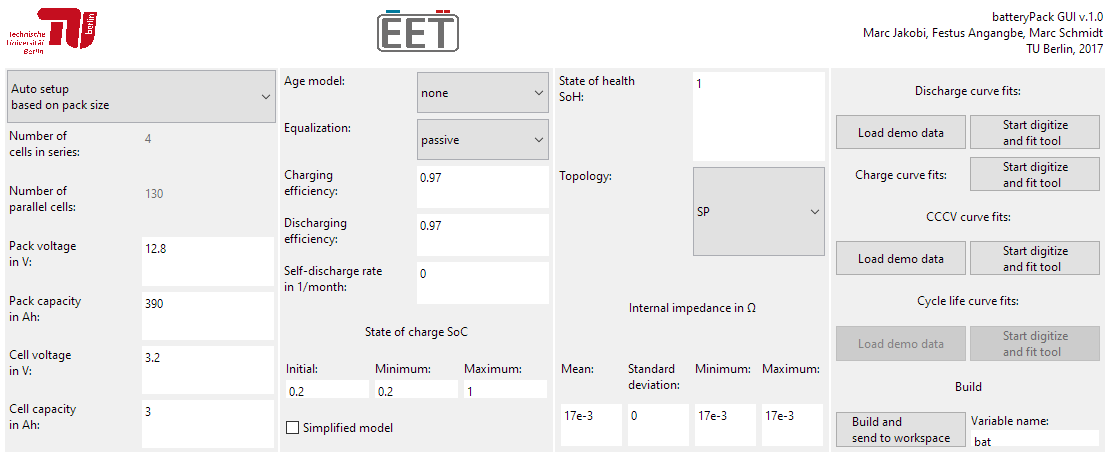
\includegraphics[width=\textwidth]{GUI.png}
			\vskip 30px
		\begin{minipage}[b]{\textwidth}
			\flushright 
			{\LARGE\textbf{Cell Resolved \matlab\ OOP Model of a Lithium Iron Phosphate Battery Pack}}\\
			\vskip 10px
			\textbf{Marc Jakobi, Festus Anyangbe, Marc Schmitdt} \\
			\today \\
			HTW Berlin \\
			\vskip 10px
			Supervision: \\ \textbf{M.Sc. Steven Neupert}\\
			TU Berlin \\
			\vskip 10px
		\end{minipage}
	\end{figure}
\end{titlepage}
\clearpage
\begin{titlepage}
	\fancypagestyle{myheadings}{Inhalt}
	\tableofcontents
\end{titlepage}\clearpage
\setcounter{page}{1}
\pagenumbering{roman}
\listoffigures
\listoftables
\section*{Acronyms}
\thispagestyle{plain}
\markboth{Acronyms}{Acronyms}
\begin{acronym}
	\acro{BMS}[BMS] battery management system
	\acro{CCCV}[CCCV] constant current / constant voltage
	\acro{EOL}[EOL] end of life
	\acro{GUI}[GUI] graphical user interface
	\acro{JVM}[JVM] \java\ virtual machine
	\acro{MEX}[MEX] \matlab\ executable
	\acro{OO}[OO] object oriented
	\acro{OOP}[OOP] object oriented programming
	\acro{SP}[SP] strings of parallel elements
	\acro{std}[std] standard deviation
	\acro{PS}[PS] parallel strings
\end{acronym}
\section*{List of symbols}
%\addcontentsline{toc}{chapter}{Formelverzeichnis} 	%Einbinden Des Verzeichnisses in das Inhaltsverzeichnis
\thispagestyle{plain}	%erste Seite des Kapitels ohne Kopfzeile
\markboth{List of symbols}{List of symbols}
\captionsetup{list=false}%captions werden nicht in die zugehörigen Verzeichnisse geschrieben

\begin{longtable}{lrl}
\captionlistentry{Symbol}\\
\toprule
Symbol		 					& Unit  	& Description \\
\midrule
								& 			&  \\
\bottomrule
\end{longtable}

\captionsetup{list=true}%captions werden in die zugehörigen Verzeichnisse geschrieben
\setcounter{table}{0}
\captionsetup{list=true}
\setcounter{table}{0}
\clearpage
\setcounter{page}{1}
\pagenumbering{arabic}


%% INCLUDES / SUBSECTIONS HERE
\markboth{Preface}{Preface}
\section*{Preface}
\addcontentsline{toc}{section}{Preface}
The following text provides a complete documentation of the battery model provided in the \mcode{lfpBattery} \matlab\ package. It combines a description of the model's components with an analysis and validation using example simulations and a tutorial on how to use the package.

\subsection*{Organization}
\addcontentsline{toc}{subsection}{Organization}
This documentation is organized in sections that are sorted in such a way that a detailed understanding of the model's design and functionality is conveyed to the reader. For a basic knowledge of how to use the model, the sections do not have to be read in order. Parts of the documentation that are not relevant to the usage of the model in \matlab\ can safely be skipped. However, it is recommended to read the entire documentation for an understanding of the strengths and weaknesses of the model.

\subsection*{Typing conventions of this documentation}
\addcontentsline{toc}{subsection}{Typing conventions of this documentation}
Since this documentation describes a \matlab\ package, the following special text formatting is used extensively:
\begin{itemize}
	\item \matlab\ code and the names of \matlab\ objects and properties are formatted in \mcode{fixed-width} font and the default \matlab\ colour coding.
	\item \matlab functions (methods) are formatted in \mcode{fixed-width} font with brackets added at the end, e.g. \mcode{plot()}.
	\item Formulas, mathematical symbols, physical units and constants are formatted according to the norms DIN~1338, DIN~1304, DIN~1301 and DIN~1313.
	\item If a formula, symbol, unit or constant is used within \matlab\ code, the \mcode{fixed-width} font is used.
\end{itemize}

\subsection*{Quick start}
\addcontentsline{toc}{subsection}{Quick start}
To quickly get started with the usage of this package, skip to the sections~\ref{sec:batteryPack} and~\ref{sec:GUI}. Note that any script or function that uses this package should start with the line
\begin{lstlisting}
import lfpBattery.*
\end{lstlisting}
Alternatively, only the required objects can be imported, e.g.
\begin{lstlisting}
import lfpBattery.batteryPack lfpBattery.dischargeCurves
bat = batteryPack(varargin{:});
dC = dischargeCurves(varargin{:});
\end{lstlisting}
or the object with the name \mcode{objectName} can be initialized as \mcode{lfpBattery.objectName}, e.g.
\begin{lstlisting}
bat = lfpBattery.batteryPack(varargin{:}); % creates a batteryPack object
\end{lstlisting}
For the code examples provided in this documentation, it is assumed that the \mcode{lfpBattery} package has been imported. \\
Section~\ref{sec:GUI} provides a description of the GUI tools that can be used for getting to know the package and for creating the required curve fits. For repeaded use in a simulation, it is recommended to start off with the \mcode{batteryPack} class, which provides centralized access to almost all of the features of this package and is described in section~\ref{sec:batteryPack}.

\subsection*{Issue Tracker}
\addcontentsline{toc}{subsection}{Issue Tracker}
To report issues, please use the GitHub issue tracker at \url{https://github.com/MrcJkb/lfpBattery/issues}

\subsection*{Terminology}
\addcontentsline{toc}{subsection}{Terminology}
Object oriented programming (OOP), design pattern and \matlab\ terminology is used frequently throughout this documentation. A short description of some of the terms is provided in the following.

\subsubsection*{Interface} \label{sec:interface}
In OOP languages such as \java and C++, the term "interface" commonly refers to an abstract set of methods that specifies the behaviour that objects must implement. Unlike a class, an interface does not have any properties. \matlab\ OOP contains abstract classes, but no interfaces. However, in the terminology of design patterns, an interface can also be an abstract class. In this documentation, an abstract class that defines the behaviour that objects must implement via a set of methods and/or properties is referred to as an "interface". Examples are the \mcode{curveFitInterface} for all curve fitting classes and the \mcode{batteryInterface}, which is a common interface for the battery pack elements and the cells.

\subsubsection*{Immutable}
In \matlab\ OOP, object properties can be private (read only) or public (read and write access), among others. A property that can be set from an object's constructor (upon initialization), but is read only afterwards is called "immutable".

\subsubsection*{Observer}
In the Observer design pattern, an observer is an object that is notified by the subject it is observing when an event occurs. The subject sends information to the observer about which event has occurred, the source of the event and which of the observer object's methods is to be triggered. Observers are also often referred to as "listeners".

\subsubsection*{Subject}
In the Observer design pattern, a subject is an object that is observed. It holds a handle reference to one or more observers and when an event occurs, it sends out a notification to the observer, triggering one or more of it's methods.

\subsubsection*{Component}
In the Composite design pattern, a component is any class that implements the shared interface. Both composite and leaf elements are components.

\subsubsection*{Composite}
In the Composite design pattern, a composite is a component that can hold a reference to another component.

\subsubsection*{Leaf}
In the Composite design pattern, a leaf is a component that cannot hold a reference to another component.
\markboth{Introduction}{Introduction}
\section{Introduction}
In recent years, energy storage has been playing a more and more important role in various sectors. With the rapid advances in lithium-ion technology, the costs of lithium-ion batteries have been decreasing and their usage increasing steadily. Today, they are applied in many fields, e.g. Electric vehicles, storage in combination with photovoltaic systems, grid stabilization, etc. The various applications result in different operation strategies and stress factors, which often need to be modelled. The modelling of batteries makes it possible to simulate the behaviour of existing technologies while designing a system (i.e. with the purpose of determining the ideal type and size of the battery). It also plays an important role in the further development of the technologies themselves (i.e. of battery management systems). \\
Most battery models can be classified into 3 categories: (i) Theoretical, (ii) semi-empirical and (iii) empirical models~\cite{cui_multi-stress_2015, xu_degradation-limiting_2013}. The most precise approach is theoretical modelling, in which it is attempted to simulate the physical processes within the battery. Such processes could be the transfer of lithium ions through the electrolyte or the ageing mechanisms, e.g. lithium plating. A negative aspect of theoretical modelling is the complexity, which results in a high resource demand and thus slow simulations. A positive aspect is the fact that theoretical models can be adapted to any type of battery. The resource demand is significantly reduced with empirical models, in which certain behaviour is represented by equivalent circuits that are parametrized from measurements. However, simplifications must be made to a certain degree and an empirical model of one battery cannot be easily transferred to another, because the measurements have to be recorded for every model. In the worst-case scenario, the measured data might differ so strongly that the model has to be changed completely. The model used in this package takes a semi-empirical approach, in which the pros of the theoretical and empirical approaches are combined. The only con is the necessity of simplifications. Theoretical phenomena are used to model measured data, which allows for easy adaptation of the model to different technologies with low resource consumption. \\
A motivation for this project is the scarcity of detailed, cell-resolved simulation models~\cite{cordoba-arenas_control-oriented_2015} and the almost complete lack of open-source models. Furthermore, most \matlab\ simulations appear to be designed in a procedural style. Object oriented (OOP) programming in \matlab\ still seems to be a rare phenomenon today, although advanced OOP capabilities were introduced as early as version R2008a~\cite{foti_inside_2008}. This may in part be due to the fact that Matlab classes are often thought of as slow (with long method overhead times). However, the just-in-time compiler\footnote{Matlab's code execution mechanism.} (JIT) was overhauled in \matlab\ R2016a, resulting in an OOP performance increase of up to 40~\% compared to the predecessor~\cite{_matlab_2016}. It can be assumed that OOP performance will only increase further with newer releases. The approach chosen for this open-source model combines the flexibility of OOP design patterns with Matlab's highly optimized double-precision general matrix-matrix multiplication (dgemm) and vectorization libraries.
\markboth{Discharge curves}{Discharge curves}
\section{Discharge curves}
\label{sec:dischargeCurvesMain}
Many battery data sheets provide measured discharge curves, on which the charging and discharging behaviour of this model is based. Rather than determining the curves according to the internal impedance, a common approach \cite{lijun_gao_dynamic_2002}, this model determins the curves directly by means of digitizing the images and creating a curve fit. The classes used for fitting and modelling the discharge curves are described in the following subsections.

\subsection{Single discharge curve}
\label{sec:dischargeFit}
For modelling a single discharge curve, the class \mcode{dischargeFit} is used, which implements the interface \mcode{curveFitInterface}\todo{Section describing interface, etc.}. The curve is fitted according to \cite{werder_entwicklung_2014}, using a function that is loosely based on the Nernst equation with two exonential functions superimposed as a correction for the voltage drops at the beginning and end of the curve.
\begin{equation}
\begin{aligned}
V(SoC) = x_1 - \frac{R\cdot T}{z\subi{Li}\cdot F}\cdot ln\Big(\frac{SoC}{1-SoC}\Big)
+ x_2\cdot SoC + x_3 \\
+ (x_4 + (x_5 + x_4\cdot x_6)\cdot SoC)\cdot exp(-x_6\cdot SoC) \\
+ x_7\cdot exp(-x_8\cdot SoC)
\end{aligned}
\end{equation}

where $x_1,\ ..,\ x_8$ are the fit parameters, $R = 8.3144598$ J/(mol $\cdot$ K) is the universal gas constant, $z\subi{Li} = 1$ is the ionic charge number of lithium, $F = 96485.3328959$ As/mol is the Faraday constant, $SoC$ is the state of charge, $V$ is the voltage in V and $T$ is the temperature in K at which the curve was recorded. The curves are fitted using the levenberg-marquardt algorithm and either the \mcode{lsqcurvefit} method, the \mcode{fminsearch} method or a combination of both, depending on the user's preference. 

\subsubsection{Creation of a \mcode{dischargeFit} object}
\label{sec:dischargeFit_creation}
A \mcode{dischargeFit} object is created with the digitized raw data - the voltage $V$ in V, the discharge capacity $C\subi{dis}$ in Ah, the current $I$ in A at which the curve was recorded and the temperature $T$ in K at which the curve was recorded.
\begin{lstlisting}
d = dischargeFit(V, C_dis, I, T);
\end{lstlisting}
\mcode{V} and \mcode{C_dis} are vectors containing the digitized raw data from the data sheet. Further options, such as initial values for the fit parameters $x_1,\ ..,\ x_8$ and the fit method can be passed to the constructor using Matlab's name-value pair syntax:
\begin{lstlisting}
d = dischargeFit(V, C_dis, I, T, 'OptionName', OptionValue);
\end{lstlisting}
By default, the initial fit parameters are set to zero and the curve is fit by first using \mcode{lsqcurvefit}, followed by \mcode{fminsearch}. The initial fit parameters are stored in a vector \mcode{x0} of \mcode{length} 8, which can be passed via the option name \mcode{'x0'}, for example using the following syntax:
\begin{lstlisting}
x0 = ones(8, 1);
d = dischargeFit(V, C_dis, I, T, 'x0', x0);
\end{lstlisting}
The method used for the curve fitting can be passed to the constructor using the option name \mcode{'mode'}. The corresponding value must be one of the following three strings:
\begin{itemize}
	\item \mcode{'lsq'} for \mcode{lsqcurvefit}
	\item \mcode{'fmin'} for \mcode{fminsearch}
	\item \mcode{'both'} for \mcode{lsqcurvefit} followed by another fit using \mcode{fminsearch}
\end{itemize}
e.g.
\begin{lstlisting}
d = dischargeFit(V, C_dis, I, T, 'mode', 'fmin');
d.plotResults
\end{lstlisting}
Depending on the curve and on the technology, one of the methods may return a better result.

\subsubsection{Visual validation}
A visual validation can be performed by calling the class's \mcode{plotResults} method (see above). In Figure~\ref{fig:dischargeFit01}, the results of two \mcode{dischargeFit} objects using the same raw data are compared.
\begin{figure}[b!]
	\captionsetup{type=figure}
	\centering
	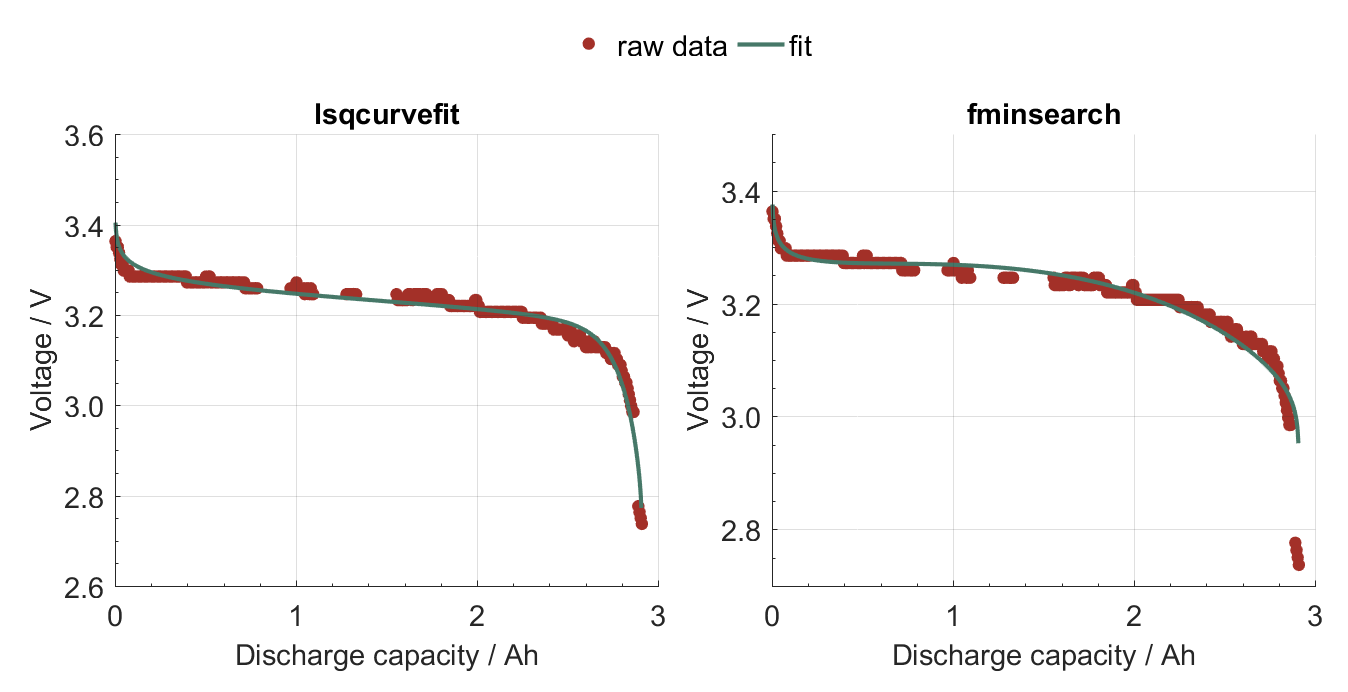
\includegraphics[width=.97\textwidth]{dischargeFit01}
	\caption[Fit results of the \mcode{dischargeFit} class using the fit methods \mcode{lsqcurvefit} and \mcode{fminsearch}, respectively]{Fit results of the \mcode{dischargeFit} class using the fit methods \mcode{lsqcurvefit} and \mcode{fminsearch}, respectively. The raw data was extracted from \cite{_data_2010}.}
	\label{fig:dischargeFit01}
\end{figure}
\begin{figure}[t!]
	\captionsetup{type=figure}
	\centering
	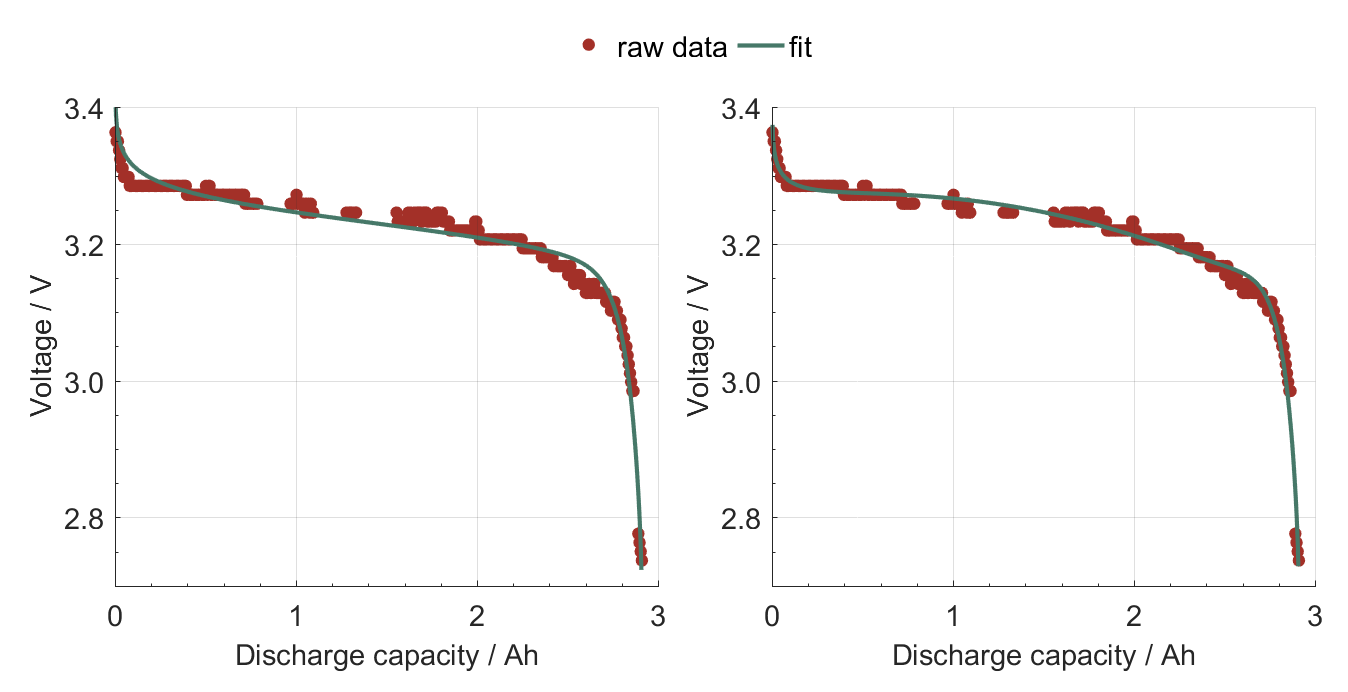
\includegraphics[width=.97\textwidth]{dischargeFit02}
	\caption[Fit results of the \mcode{dischargeFit} class using the fit mode \mcode{'both'} with the default parameter initialization and with a custom parameter initialization]{Fit results of the \mcode{dischargeFit} class using the fit mode \mcode{'both'} with the default parameter initialization (left) and with a custom parameter initialization (right). The raw data was extracted from \cite{_data_2010}.}
	\label{fig:dischargeFit02}
\end{figure}

In this example, \mcode{'lsq'} appears to return better results for the voltage drop at the end of the curve, while \mcode{'fmin'} results in a more precise fit for the voltage drop at the beginning of the curve. Further differences can be seen in the fits' curvatures. 
The \mcode{'lsq'} option results in a slightly flatter curve than the \mcode{'fmin'} mode. The results of a \mcode{dischargeFit} object using the \mcode{'both'} option are presented in Figure~\ref{fig:dischargeFit02}.
Using the default fit parameter initialization of \mcode{zeros} (left) appears to improve the curvature and voltage drops slightly, compared to the other modes. Further improvements can be made by passing custom initial fit parameters to the constructor via the option \mcode{'x0'} (see Figure~\ref{fig:dischargeFit02}, right).

\subsubsection{Object properties}
Further fit quality analysis can be performed via the mean difference in voltage between the raw data and the curve fit at the respective positions of the raw data $\overline{\Delta V}$ in V and the maximum difference between the raw data and the curve fit at the respective positions $\Delta V\subi{max}$ in V. Additionally, every curve fit class (i.e. \mcode{dischargeCurves}, \mcode{woehlerFit}, etc.) in this package implements the \mcode{curveFitInterface}, which contains the root mean square error $rmse$ as a property.
The $rmse$ for a curve fit with the raw data $y\subi{raw}$ and the fitted data $y\subi{fit}$ at the same respective $x$ coordinates is defined as
\begin{equation}
rmse = \sqrt{\frac{\sum_{i = 1}^{n}(|y\subs{raw}{i}-y\subs{fit}{i}|)^2}{n}}
\end{equation}
where $i$ is the index of the measurement and $n$ is the number of measurements. In the case of a \mcode{dischargeFit} object, $y\subs{raw}{i}$ is the measured voltage at the discharge capacity $C\subs{dis}{i}$ and $y\subs{fit}{i}$ is the fitted voltage at $C\subs{dis}{i}$. Often used for forecasting models, the $rmse$ provides a good measure of accuracy when comparing two models of the same data set~\cite{hyndman_another_2006}.
In the previous examples, the curve fit using the \mcode{'lsq'} method (Figure~\ref{fig:dischargeFit01}, left) has an $rmse$ of 0.0244~V. Using the \mcode{'fmin'} mode (Figure~\ref{fig:dischargeFit01}, right) improves the $rmse$ to a value of 0.0162~V and using the fit mode \mcode{'both'} (Figure~\ref{fig:dischargeFit02}, left) further improves it to 0.0157~V.  The lowest $rmse$ (0.0106~V) is achieved with the custom fit parameter initialization (Figure~\ref{fig:dischargeFit02}, right). \\
A list of the class's accessible properties is provided in Table~\ref{tab:dischargeFitProps}. The \mcode{z} property is inherited from the \mcode{curveFitInterface}. Setting the \mcode{x} or \mcode{mode} properties will cause the object to re-run the fitting algorithm, thus likely resulting in different values for \mcode{x} than were set by the user.

\begin{table}%[b]
	\centering
	\caption[Accessible properties of the \mcode{dischargeFit} class]{Accessible properties of the \mcode{dischargeFit} class.}
	\begin{tabular}{llll}
		\toprule
		Name & Description & Unit & Set access \\
		\midrule
		\mcode{x} & 8x1 vector of fit parameters & - & public \\
		\mcode{dV_mean} & Mean voltage difference between raw data and fit & V & read only \\
		\mcode{dV_max} & Max voltage difference between raw data and fit & V & read only \\
		\mcode{T} & Temperature at which the curve was recorded & K & immutable \\
		\mcode{z} & Current of the curve & A & immutable \\
		\mcode{mode} & Method used for fitting (\mcode{'fmin'}, \mcode{'lsq'} or \mcode{'both'})& - & public \\
		\mcode{rmse} & Root mean square error & V & read only \\
		\bottomrule
	\end{tabular}
	\label{tab:dischargeFitProps}
\end{table}

\subsubsection{Usage of a \mcode{dischargeFit} object}
In order to calculate a voltage for a given discharge capacity, the object can be treated like a function handle, by using \mcode{subsref} indexing.
\begin{lstlisting}
d = dischargeFit(V, C_dis, I, T, 'mode', 'fmin');
Cd = 1.5; % Discharge capacity in Ah
V = d(Cd); % Voltage in V
Cd_vect = linspace(0, 3, 1000); % Vector of discharge capacities in Ah
V_vect = d(Cd_vect); % Corresponding vector of voltages in V
\end{lstlisting}
A \mcode{dischargeFit} object is not accessed directly by the battery model, but rather stored in a \mcode{dischargeCurves} object. After creating a \mcode{dischargeFit}, it can be added to a \mcode{dischargeCurves} collection by using the \mcode{add()} method (see section~\ref{sec:dischargeCurves}). Alternatively, it can be added directly to a subclass of the \mcode{batteryInterface} (see section) \todo{section ref} using it's \mcode{addcurves()} method. \\

\subsection{Collection of discharge curves}
\label{sec:dischargeCurves}
A single discharge curve can be used to model the behaviour of a battery for a given current. However, in reality, a battery will often be charged or discharged with different currents. In many cases, the current may change from one simulation time step to another. In order to be able to determine the voltage as a function of $C\subi{dis}$ and $I$, multiple \mcode{dischargeFit} objects are wrapped by a \mcode{dischargeCurves} object, which is described in the following sections.

\subsubsection{Creation of a \mcode{dischargeCurves} object}
There are two ways to initialize a \mcode{dischargeCurves} object. The first option is to create an empty object and using the class's \mcode{dischargeFit()} method to add curve fits. The \mcode{dischargeFit()}  method has the same syntax as the \mcode{dischargeFit} class's constructor.
\begin{lstlisting}
dC = dischargeCurves;
I = [0.6; 1; 3; 5; 10; 20]; % Vector of currents in A
T = 293; % Temperature in K
for i = 1:6
	dC.dischargeFit(raw(i).V, raw(i).Cd, I(i), T)
end
% raw is a struct array containing the measured curve data
% from the data sheet.
\end{lstlisting}
This option has the advantage of reducing clutter in the workspace. However, changing the parameters and analysing the accuracy of the individual curve fits is more complicated.
Alternatively, the \mcode{dischargeFit} objects can be created, modified and then passed to the \mcode{dischargeCurves} constructor.
\begin{lstlisting}
d1 = dischargeFit(raw(1).V, raw(1).Cd, I(1), T);
	% Quality analysis and fit perfection here...
	% More curve dischargeFit object initializations here...
d6 = dischargeFit(raw(6).V, raw(6).Cd, I(6), T);
	% Quality analysis and fit perfection here...
dC = dischargeCurves(d1, d2, d3, d4, d5, d6);
% Equivalent:
dC = dischargeCurves;
dC.add(d1)
dC.add(d2)
% ...
dC.add(d6)
\end{lstlisting}
If a \mcode{dischargeFit} is passed to a \mcode{dischargeCurves} object that already holds a reference to a \mcode{dischargeFit} with the same current, the stored reference is replaced by the new one. Similarly, if two or more \mcode{dischargeFit} objects with the same current are passed to a \mcode{dischargeCurves} constructor, the first one is ignored.

\subsubsection{Interpolation between curves}
The calculation of the voltage for any given current and discharge capacity is done via Matlab's built-in \mcode{griddedInterpolant} class, which is called from within the \mcode{interp()} method. The syntax for a \mcode{dischargeCurves} object \mcode{dC} is as follows:
\begin{lstlisting}
V = dC.interp(I, Cd);
V = interp(dC, I, Cd); % equivalent
\end{lstlisting}
Where \mcode{V} is the voltage in V, \mcode{I} is the charging or discharging current in A and \mcode{Cd} is the discharge capacity after charging or discharging in Ah. If \mcode{I} is equal to one of the stored \mcode{dischargeFit} objects' currents, \mcode{Cd} is simply passed on to the respective object, which returns the voltage. If \mcode{I} does not match any of the stored objects and either of the input arguments is not found in the object's cache, \mcode{Cd} is passed on to each of the stored \mcode{dischargeFit} references, creating a vector of voltages for the different currents. Finally, a \mcode{griddedInterpolant} is created using the sample points, \mcode{I} is passed to it and the interpolated voltage is returned and cached. The interpolation method (the default is \mcode{'spline'}) can be changed by setting the property \mcode{interpMethod}. \\
A visual validation of the interpolation using the \mcode{'linear'} and \mcode{'spline'} methods, respectively, is depicted in Figure~\ref{fig:interpMethod}. A collection of \mcode{dischargeFit} objects for six currents was created and the fit results were plotted. Then, all fits except for the one at 10~A were added to a \mcode{dischargeCurves} object. Finally, the \mcode{interp()} method was called for a current of 10~A and a range of discharge capacities, in an attempt to replicate the \mcode{dischargeFit} results using interpolation. The linearly interpolated curve (Figure~\ref{fig:interpMethod}, left) is almost identical to the fit until the beginning of the voltage drop at the end. 
\begin{figure}[hbt!]
	\captionsetup{type=figure}
	\centering
	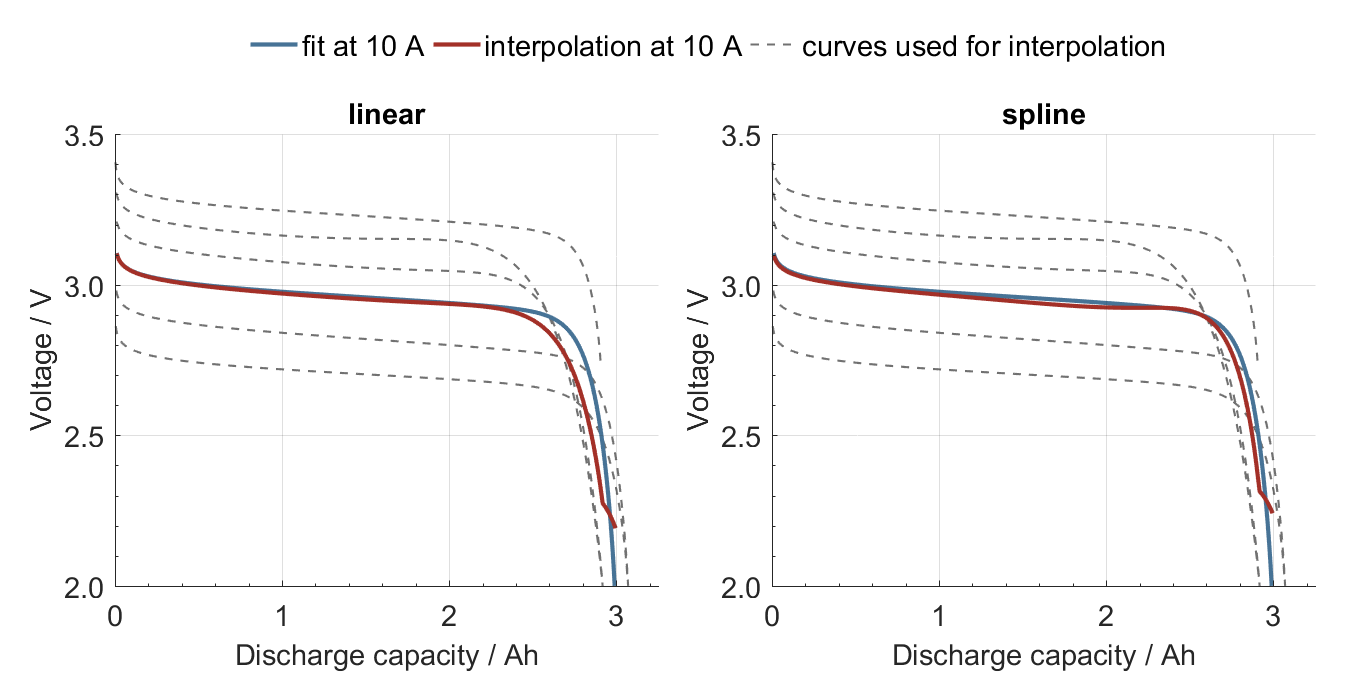
\includegraphics[width=.97\textwidth]{interpMethod}
	\caption[Comparison of the \mcode{dischargeCurves} results using linear interpolation and spline interpolation, respectively]{Comparison of the \mcode{dischargeCurves} results using linear interpolation and spline interpolation, respectively. The raw data was extracted from \cite{_data_2010}.}
	\label{fig:interpMethod}
\end{figure}
However, the spline interpolation results in an overall more precise replication of the fit if the entire curve is regarded. This indicates that the most suitable interpolation method may depend on the maximum depth of discharge $DoD$ of the modelled battery. As can be seen in Figure~\ref{fig:interpMethod}, the interpolation bends slightly at the end of the curve (close to a discharge capacity of 3~Ah). This is due to the fact that the voltage returned by a \mcode{dischargeFit} object is limited to the minimum and maximum of the raw data, respectively. If it were not limited, it could return \mcode{-Inf} or \mcode{Inf}, causing the interpolation to fail. Since most lithium ion batteries' $DoD$ are limited to 0.8 or 0.9, this bend should rarely cause any issues. \\
\begin{figure}[t!]
	\captionsetup{type=figure}
	\centering
	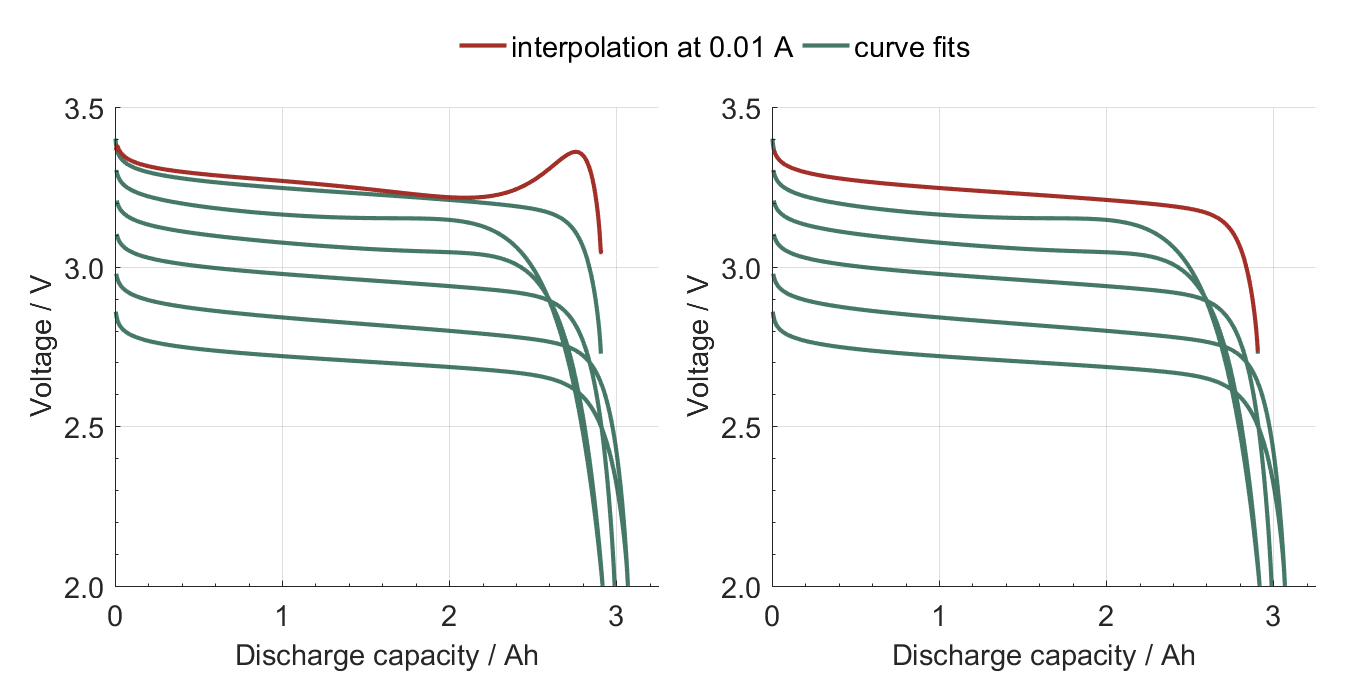
\includegraphics[width=.97\textwidth]{dischargeCurvesIlim}
	\caption[Result of the \mcode{interp()} method for a current below the lowest measured current without output limitation and with output limitation]{Result of the \mcode{interp()} method for a current below the lowest measured current without output limitation (left) and with output limitation (right). The raw data was extracted from \cite{_data_2010}.}
	\label{fig:dischargeCurvesIlim}
\end{figure}
As demonstrated Figure~\ref{fig:dischargeCurvesIlim} (left), the \mcode{interp} method using spline interpolation does not provide a good extrapolation of currents. In order to correct this, the voltage output is limited by the curve fit with the lowest current $I\subi{min}$ and by the curve fit with the highest current $I\subi{max}$, respectively. As a result, the \mcode{dischargeFit} recorded at $I\subi{min}$ is called for any current below $I\subi{min}$ (see Figure~\ref{fig:dischargeCurvesIlim}, left) and the \mcode{dischargeFit} recorded at $I\subi{max}$ is called for any current above $I\subi{max}$. In this model, the battery's maximum discharging current is limited by the \mcode{dischargeCurves} object's $I\subi{max}$ (see section\todo{ref section}).

\subsubsection{Usage of a \mcode{dischargeCurves} object}
Similarly to a \mcode{dischargeFit}, the results of a \mcode{dischargeCurves} object can be visually validated using the \mcode{plotResults()} method. Individual curve fit references removed using the \mcode{remove()} method and the respective currents. \clearpage
\begin{lstlisting}
% d = dischargeFit object
% I = current
dC.add(d) % add d to dischargeCurves dC
dC.remove(I) % remove the dischargeFit object with current I from dC
\end{lstlisting}
In order to access the \mcode{dischargeFit} references stored within a \mcode{dischargeCurves} object, the \mcode{createIterator()} method can be used. This creates an iterator object, a \matlab\ implementation of the \mcode{java.util.iterator} interface~\cite{_iterator_????}. The object can be used to iterate through the wrapped \mcode{dischargeFit} objects using a similar syntax to that of a \java\ iterator.
\begin{lstlisting}
it = dC.createIterator; % returns an scIterator object
while it.hasNext % returns true if there is another object to
				 % iterate through
	d = it.next; % returns a dischargeFit object
	% more code here
end
it.reset % resets the scIterator
\end{lstlisting}
For usage in a battery model, a \mcode{dischargeCurves} object is passed to an implementation of the \mcode{batteryInterface} (see section\todo{ref section}) using it's \mcode{addCurves()} method.
\markboth{Age model}{Age model}
\section{Age model}
The age model is implemented using the Observer design pattern via Matlab's "Events and Listeners\footnote{in \matlab, an observer is often referred to as a "listener". However, "observer" is the more common term in OOP design pattern terminology and will be used throughout this documentation.}"~\cite{_overview_????}. This way, various age models (predefined or custom) can be dynamically added to a battery model at run time or even left out completely. Ageing can be simulated on the battery pack level (by treating all cells as one entity) or on the cell level (by observing each cell separately)\footnote{see section}\todo{ref section in footnote}. The event oriented age model provided in this package is based solely on cycle counting, for which a mathematical approach developed by~\cite{dambrowski_mathematical_2012} is implemented. Descriptions of the counting algorithm and the classes used to implement the age model are provided in the following sections.
\subsection{Overview}
Cycle counting algorithms are designed to count cycles from a set of measured data. A challenge for a running simulation or a battery management system (BMS) that relies on cycle counting is to decide when to count the cycles of an accumulated data set. Counting could be done at fixed time intervals or it could be triggered by a certain event. The latter is the approach implemented by the \mcode{cycleCounter} interface, which acts both as an observer of a battery cell or pack as well as a subject for the \mcode{eoAgeModel} class.\\
The observation of charge cycles is handled by the abstract \mcode{cycleCounter} interface, in which all methods except for the \mcode{count()} method are predefined. An object that implements the interface is regularly updated with the observed battery's $SoC$, which is stored within the object's memory. The cycle counting occurs every time the $SoC$ reaches an upper threshold, i.e. the observed battery's maximum $SoC$. After counting, the \mcode{NewCycle} event is triggered, causing all of the object's observers (i.e. an \mcode{eoAgeModel} object) to be notified that new data is available for simulation. The age model then uses the data to determine the battery's new state of health $SoH$ and passes it on to the battery. \\
An Observer Pattern class diagram of the age model is depicted in Figure~\ref{fig:observer_schema}. The observation is handled by the respective abstract interfaces, while the actual simulation is handled by the implementations. This makes the model highly flexible. For example, a lightweight implementation could be to observe a \mcode{batteryPack} using a single \mcode{cycleCounter} and a single \mcode{batteryAgeModel}. Another option could be to use multiple \mcode{cycleCounter} and \mcode{ageModel} objects in order to simulate the ageing of each \mcode{batteryCell} within a pack individually. The cycle counting can be implemented by various algorithms (two are provided in this package). And advanced users could even replace the default age model implementation (\mcode{eoAgeModel}) with a custom class that takes other factors into account, e.g. calendar ageing or thermal influences. In large simulations, it may be of interest to neglect the battery ageing in order to save simulation time. This can either be done by simply not linking up the components at runtime or by including a \mcode{dummyCycleCounter} and a \mcode{dummyAgeModel}. These classes implement the \mcode{cycleCounter} and \mcode{batteryAgeModel} interfaces, respectively. However, calling their methods does nothing. The former option is faster, due to reduced method overhead, but the latter may be more robust in some cases.
\begin{figure}[t!]
	\captionsetup{type=figure}
	\centering
	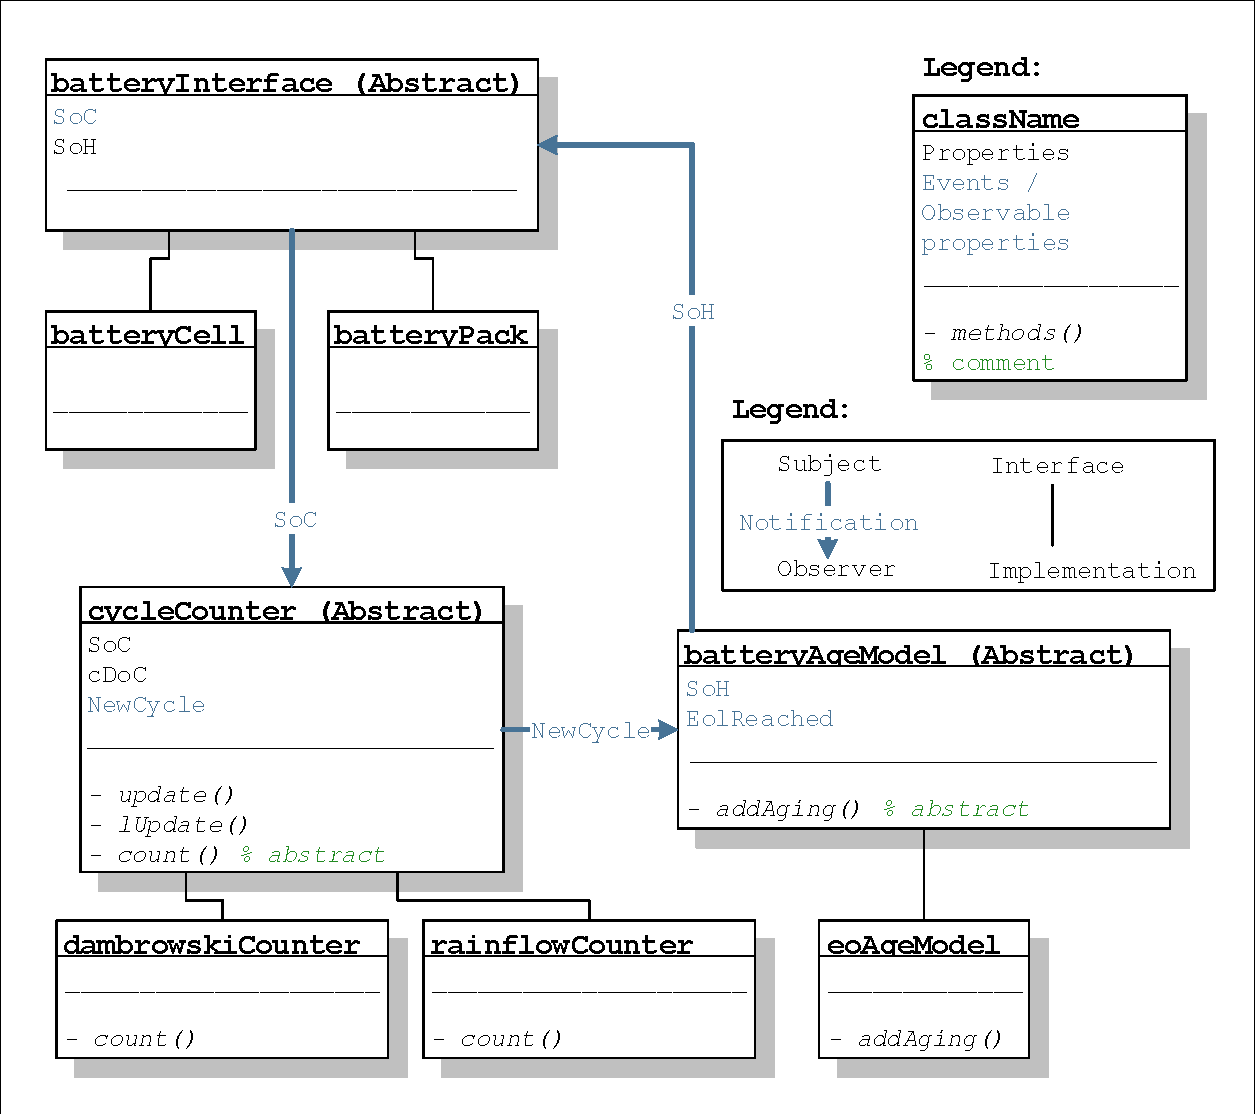
\includegraphics[width=\textwidth]{observer_schema.pdf}
	\caption[Overview of the Observer implementation of the age model with communication flows and inheritance links]{Overview of the Observer implementation of the age model with communication flows and inheritance links.}
	\label{fig:observer_schema}
\end{figure}

\subsection{Cycle counting}
In this pack, two classes have been created to implement the \mcode{cycleCounter}'s \mcode{count()} method.
A \mcode{cycleCounter} subclass can be constructed in one of the following ways:
\begin{lstlisting}
c = cycleCounter; % sets the initial SoC to 0.2 and the max. SoC to 1
c = cycleCounter(init_soc); % sets the initial SoC
c = cycleCounter(init_soc, soc_max); % sets the initial SoC and the
									 % max. SoC
\end{lstlisting}
where \mcode{cycleCounter} must be replaced with the name of the respective class that is being constructed (e.g. \mcode{dambrowskiCounter} or \mcode{rainflowCounter}). To register the object as an observer of a battery object \mcode{bat}\footnote{\mcode{bat} can be an object of any class that implements the \mcode{batteryInterface}.}\todo{ref section}, the \mcode{initAgeModel()} method can be used.
\begin{lstlisting}
% Extract intitial SoC and max. SoC from battery
init_soc = bat.SoC;
soc_max = bat.socMax;
% Replace "cycleCounter" with the respective subclass
c = cycleCounter(init_soc, soc_max);
% Intitialize event oriented age model with cycle counter c
bat.initAgeModel('ageModel', 'EO', 'cycleCounter', c)
\end{lstlisting}
Note that the \mcode{'ageModel'} option must be specified, otherwise \mcode{bat} will internally replace \mcode{c} with a \mcode{dummyCycleCounter} object to prevent runtime errors. If this happens, a warning message is printed to the command window.

\subsubsection{The \mcode{rainflowCounter} class}
The state of the art algorithm for cycle counting, "rainflow", was originally developed for mechanical stress modelling~\cite{matsuishi_fatigue_1968} and has recently become popular in the field of battery charge cycle counting~\cite{dufo-lopez_multi-objective_2008}. The \mcode{rainflowCounter} class was added to this package for the purpose of demonstrating the flexibility of the age model implementation. It acts as an adapter for the popular FileExchange contribution, "Rainflow Counting Algorithm" by Adam Nieslony~\cite{_rainflow_????}. In order for the class to work, the MEX functions must be downloaded from \cite{_rainflow_????} and placed within Matlab's search path. They are not included in this package and attempting to construct a \mcode{rainflowCounter} object will fail if they are not found. To register a \mcode{rainflowCounter} with a battery \mcode{bat}, the above syntax must be used, whereby \mcode{cycleCounter(init_soc, soc_max)} is replaced by \mcode{rainflowCounter(init_soc, soc_max)}.

\subsubsection{The \mcode{dambrowskiCounter} class}
In 2012, J.~Dambrowski, S.~Pichlmaier and A.~Jossen developed a mathematical definition of a battery's charge cycles along with an algorithm for counting them~\cite{dambrowski_mathematical_2012}. Since the counting algorithm was not named, the \mcode{dambrowskiCounter} class that implements it in this package was named after one of the authors. In their approach, so-called pre-cycles are counted and compared with each other. This is visualized in Figure~\ref{fig:pre_cycles}. The twice depicted $SoC$ curve (grey) has two local maxima $SoC\subs{max,l}{i}$, since the last value is counted as a local maximum. Starting from an $SoC\subs{max,l}{i}$, a pre-cycle of "prior equality" is defined as the $SoC$ within an interval between the respective  $SoC\subi{max,l}$ and the last point at which the $SoC$ was equal to  $SoC\subi{max,l}$. Two such pre-cycles are depicted in Figure~\ref{fig:pre_cycles} (left) and coloured in red and blue, respectively. A pre-cycle of "subsequent equality" (Figure~\ref{fig:pre_cycles}, right, coloured in blue) is defined as the $SoC$ within an interval between the respective $SoC\subi{max,l}$ and the subsequent point at which the $SoC$ is equal to $SoC\subi{max,l}$. Finally, a pre-cycle is counted as a cycle if there is no larger pre-cycle that encompasses the same interval and shares the same local minimum. This is not the case for the small cycle (coloured red) in Figure~\ref{fig:pre_cycles} (left); so the depicted curve contains two cycles. \\ \\
\begin{centering}
	\begin{figure}[t!]
		\subfloat{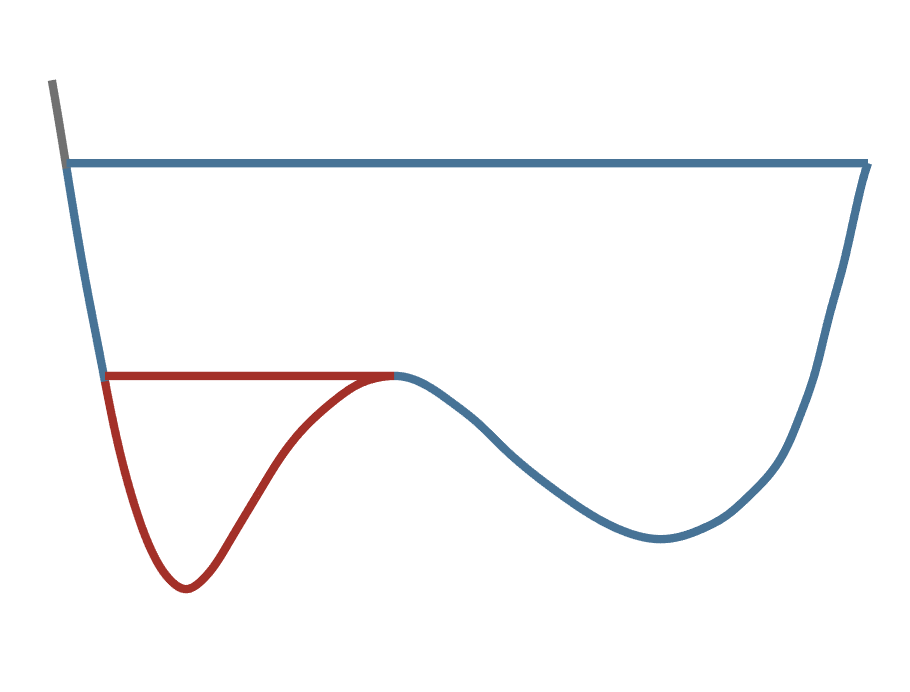
\includegraphics[width=0.5\textwidth]{DAM01}}
		\subfloat{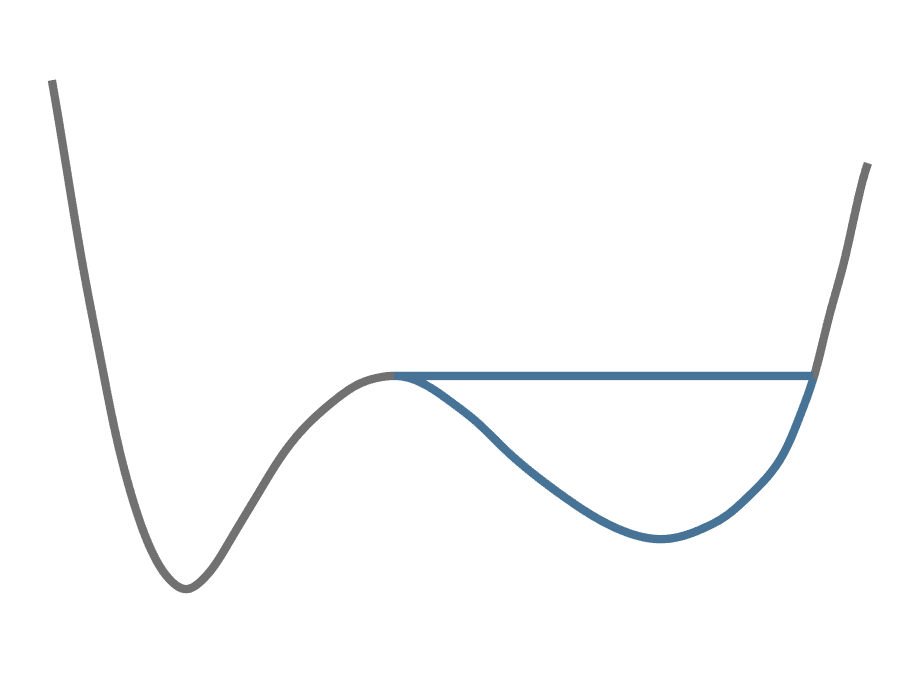
\includegraphics[width=0.5\textwidth]{DAM02}}
		\captionsetup{type = figure}
		\caption[Qualitative visualization of pre-cycle counting: Two pre-cycles of prior equality and a pre-cycle of subsequent equality]{Qualitative visualization of pre-cycle counting according to~\cite{dambrowski_mathematical_2012}: Two pre-cycles of prior equality (left) and a pre-cycle of subsequent equality (right).}
		\label{fig:pre_cycles} 
	\end{figure}
\end{centering}
In this package, \mcode{dambrowskiCounter} is the default cycle counter if an age model is specified. Thus, it does not have to be passed as an argument in a battery's \mcode{initAgeMode()} method.
\begin{lstlisting}
bat.initAgeModel('ageModel', 'EO')
% Automatically initializes a dabrowskiCounter object with init_soc
% and soc_max set according to the battery's properties and links.
\end{lstlisting}

\subsubsection{Comparison of the cycle counters}
Each \mcode{cycleCounter} object's \mcode{count()} method converts the saved $SoC$ profile into a cycle-Depth-of-Cycle $cDoC$ curve - a vector containing the depths of discharge $DoD$ of all the counted cycles. The simulation results of two batteries using a \mcode{dambrowskiCounter} and a \mcode{rainflowCounter}, respectively, are compared in Figure~\ref{fig:cdoc_hists}. The cycles' $DoD$s are each sorted into 50 BINs and compared in a histogram. Overall, the histograms appear very similar, thus proving that both classes produce good results. However, more cycles are counted using the \mcode{dambrowskiCounter} class, possibly causing the simulated battery to age slightly faster. While both classes use different methods for determining the extrema\footnote{\mcode{dambrowskiCounter} uses \mcode{cycleCounter}'s \mcode{iMaxima()} method and \mcode{rainflowCounter} uses the \mcode{sig2ext()} function~\cite{_rainflow_????}.}, the amount local maxima found is the same. Thus, the determination of extrema can be ruled out as a cause and the root of the discrepancy must lie within the different counting approaches.
\begin{figure}[t!]
	\captionsetup{type=figure}
	\centering
	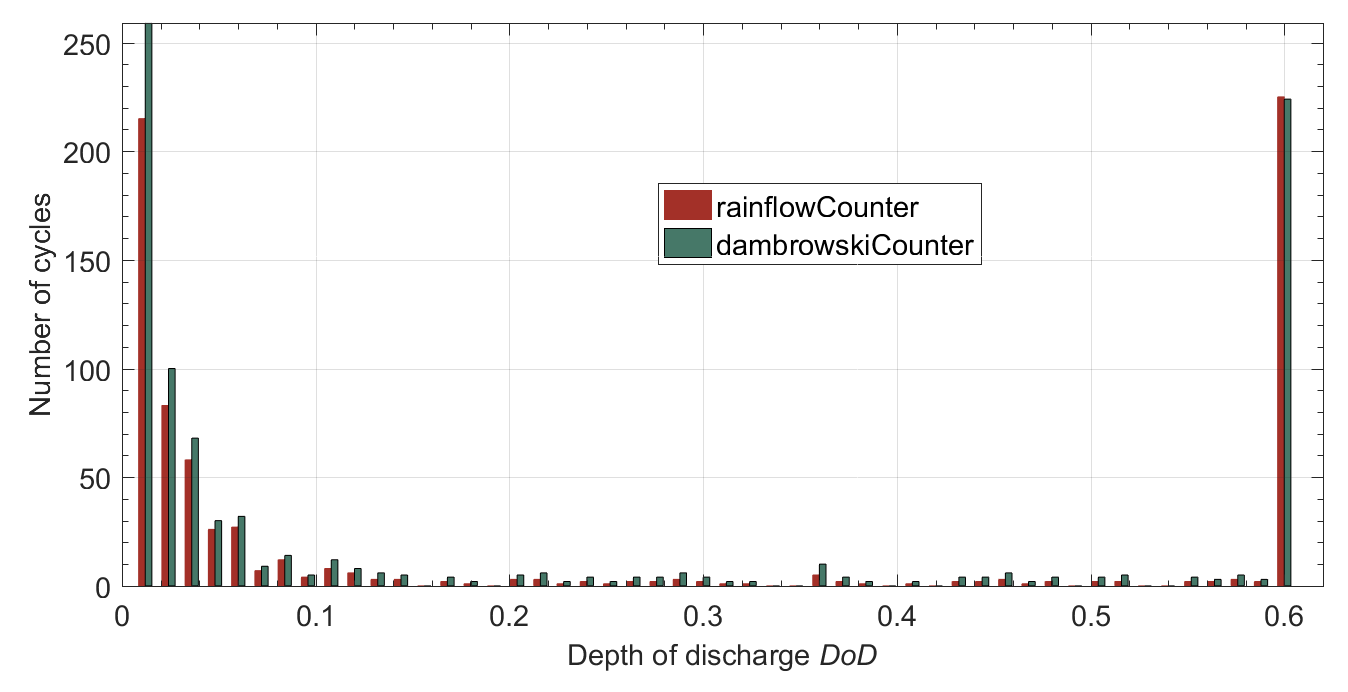
\includegraphics[width=\textwidth]{cdoc_hists}
	\caption[Comparison of the counted cycles and their $DoD$ between two simulations using the \mcode{rainflowCounter} and the \mcode{dambrowskiCounter} using the same $SoC$ profile]{Comparison of the counted cycles and their $DoD$ between two simulations using the \mcode{rainflowCounter} and the \mcode{dambrowskiCounter} using the same $SoC$ profile.}
	\label{fig:cdoc_hists}
\end{figure}

\subsection{Event oriented ageing model}
The event oriented ageing model - a very simple and lightweight model - is implemented by the \mcode{eoAgeModel} class, which subclasses the abstract \mcode{batteryAgeModel} interface. Cycle ageing is calculated based on a curve fit of the battery's number of cycles to failure $N\subi{f}$ vs $DoD$ curve.

\subsubsection{Cycle life curve fits}
Due to the fact that the cycle ageing can vary strongly between technologies, it can be difficult to find a good fit for the $N\subi{f}$ vs $DoD$ curve. In order to provide some flexibility, three different classes, each implementing the \mcode{curveFitInterface}, are provided for fitting such curves in this package: \mcode{woehlerFit}, \mcode{nrelcFit} and \mcode{deFit}.
They only differ in their class names, the number of fit parameters and in the functions used for fitting. The function used in \mcode{woehlerFit} is based on a metal fatigue curve (also known as a "W{\"o}hler curve")~\cite{naumann_betriebsabhangige_2014}
\begin{equation}
N\subi{f}(DoD) = x\subi{1}\cdot DoD^{-x\subi{2}}
\end{equation}
with the fit parameters $x\subi{1}$ and $x\subi{2}$. The \mcode{nrelcFit} class bases it's fit method on an older model \cite{drouilhet_battery_1997}.
\begin{equation}
N\subi{f}(DoD) = x\subi{1}\cdot \frac{1}{DoD}\cdot exp\bigg(x\subi{2}\cdot \bigg(1 - \frac{1}{DoD}\bigg)\bigg)
\end{equation}
Finally, the \mcode{deFit} class uses a double exponential function that was originally developed for lead-acid batteries~\cite{bindner_lifetime_2005}. However, it also seems to provide decent results for lithium-ion batteries in some cases.
\begin{equation}
N\subi{f}(DoD) = x\subi{1} + x\subi{2}\cdot exp(-x\subi{3}\cdot DoD) + x\subi{4}\cdot exp(-x\subi{5}\cdot DoD)
\end{equation}
An example for the fit results of a \mcode{woehlerFit} object is depicted in Figure~\ref{fig:woehlerFit}. Due to a lithium-ion battery's extremely large amount of cycles to failure at low $DoD$s, large relative errors may occur, especially at $DoD$s close to 1. In order to reduce the $rmse$, as many raw data points as possible should be provided for fitting. \\
\begin{figure}[t!]
	\captionsetup{type=figure}
	\centering
	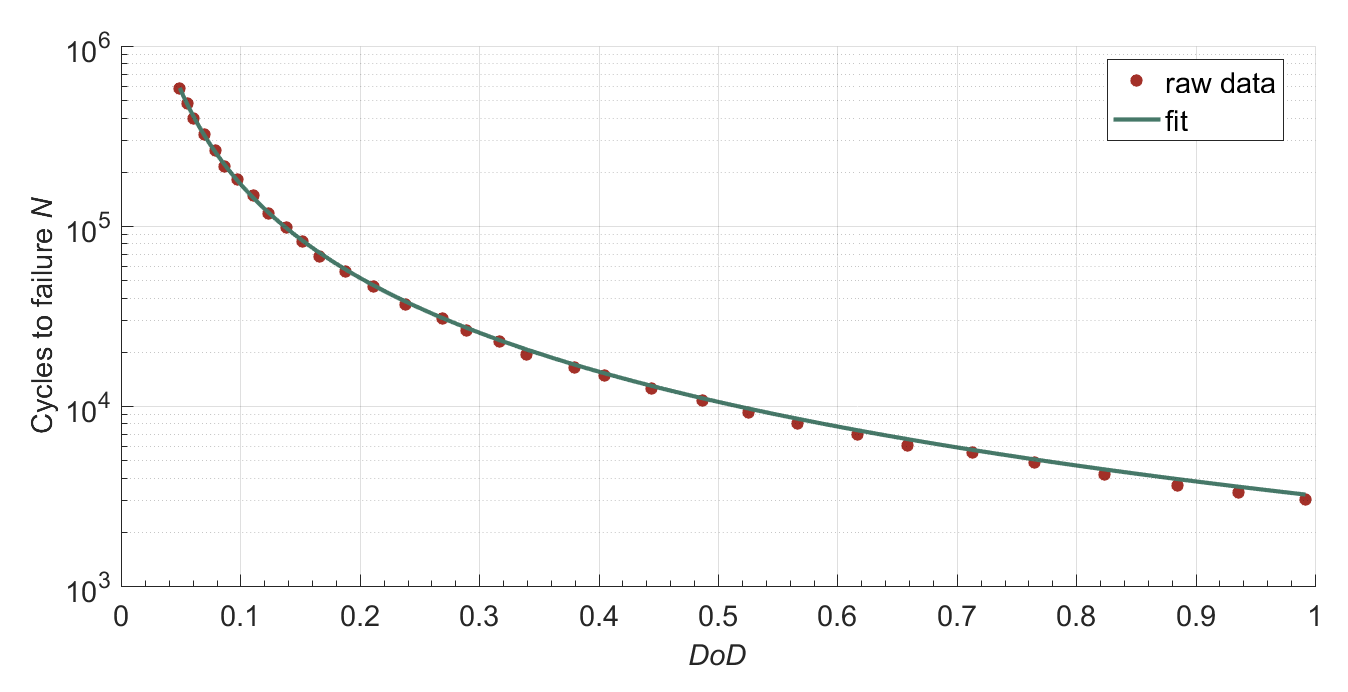
\includegraphics[width=\textwidth]{woehlerFit}
	\caption[Example for a lithium ion battery's $N\subi{f}$ vs $DoD$ cycle life curve fitted using the \mcode{woehlerFit} class]{Example for a lithium ion battery's $N\subi{f}$ vs $DoD$ cycle life curve fitted using the \mcode{woehlerFit} class.}
	\label{fig:woehlerFit}
\end{figure}
A cycle life curve fit object is initialized with the raw data and the optional name-value pairs that the \mcode{dischargeFit} and every other subclass of the \mcode{curveFitInterface} accepts (see section~\ref{sec:dischargeFit_creation}). It can then be passed on to an age model via it's constructor or by setting it's \mcode{wFit} property.
\begin{lstlisting}
% DoD = depth of discharge, N = number of cycles to failure
fit1 = woehlerFit(DoD, N);
% Plot results to new figure window
fit1.plotResults;
% Example using lsqcurvefit
fit2 = deFit(DoD, N, 'mode', 'lsq');
% Example using fminsearch and with custom initial params
fit3 = nrelcFit(DoD, N, 'mode', 'fmin', 'x0', [0.5; 1]);
% Pass cycle counter cy and fit1 to age model via it's constructor
am = eoAgeModel(cy, fit1);
% Replace fit1 with fit2 in age model
am.wFit = fit2;
\end{lstlisting}
\clearpage
Alternatively, a cycle life curve fit can be passed directly to a battery object \mcode{bat} via it's \mcode{addcurves()} method.
\begin{lstlisting}
fit = woehlerFit(DoD, N);
bat.initAgeModel('ageModel', 'EO')
bat.addcurves(fit, 'cycleLife')
\end{lstlisting}
If the age model has not been initialized when the curve fit is added, it is stored for later use.
\begin{lstlisting}
bat.addcurves(fit, 'cycleLife')
bat.initAgeModel('ageModel', 'EO') % fit is automatically passed
% to the age model
\end{lstlisting}
As well as curve fit objects, function handles to functions of one variable are accepted. However, anonymous functions are not recommended, due to their significant performance penalty.
\begin{lstlisting}
fit = @(x)(3000 * x.^(-1.73));
bat.addcurves(fit, 'cycleLife')
\end{lstlisting}

\subsubsection{Cycle ageing}
A battery's age $A\subi{c}$ is the opposite of the $SoH$, which is the usable capacity $C\subi{bu}$ divided by the nominal capacity $C\subi{n}$.
\begin{equation}
\label{eq:age_soh}
A\subi{c} = 1 - SoH = 1 - \frac{C\subi{bu}}{C\subi{n}}
\end{equation}
In the \mcode{eoAgeModel} class, the ageing due to cycling stress $A\subi{cyc}$ with $n$ cycles and their respective $DoD$ is determined from the curve fit $N\subi{f}(DoD)$.
\begin{equation}
A\subi{cyc} = \sum_{i=1}^{n}\frac{1}{N\subi{f}(DoD_i)}
\end{equation}
Every time a set of cycles is counted, $A\subi{cyc}$ is determined and added to $A\subi{c}$. 

\subsubsection{Age model initialization}
The default constructor syntax of a \mcode{batteryAgeModel} is as follows:
\begin{lstlisting}
am = batteryAgeModel; % Replace batteryAgeModel with the subclass name
% eoAgeModel requires at least one input (a cycle counter cy)
am = eoAgeModel(cy);
am = eoAgeModel(cy, cfit); % adds a cycle life curve fit
% Specify the SoH at which the end of life is reached (default: 0.2)
am = eoAgeModel(cy, cfit, soh_eol);
am = eoAgeModel(cy, cfit, soh_eol, soc_ini); % Set the initial SoC
\end{lstlisting}
To initialize the age model directly from a battery \mcode{bat}, use it's \mcode{initAgeModel()} method.
\begin{lstlisting}
bat.initAgeModel('ageModel', 'EO') % default eoAgeModel
\end{lstlisting}

\subsubsection{Creating a user-defined age model}
\label{sec:userAgeModel}
The \mcode{eoAgeModel} class does not take into account calendar ageing, which may be needed in some cases. It was left out of the default class because in many cases, a weighted degradation factor may be sufficient. The following source code snippet provides an example of how the \mcode{eoAgeModel} could be subclassed to extend it with a simple calendar ageing model. A property which holds the battery's calendar life is added and initialized in the constructor, taking into account the end of life age (typically 0.2). Finally, an \mcode{addCalAge()} method is added, that calculates calendar ageing as a linear function of the time step size. This method can be called from within the main simulation. To create a completely different age model (i.e. one that takes thermal influences into account), subclass the \mcode{batteryAgeModel} class instead.
\begin{lstlisting}
classdef myCalendarAgeModel < lfpBattery.eoAgeModel
%MYCUSTOMAGEMODEL: An example for a user-defined age model.
%Combines the event oriented age model with a linear calendar age model.

	properties
		L_cal; % calendar life in s
	end
	
	methods
		function obj = myCalendarAgeModel(l, varargin)
			% l = calendar life in years
			% varargin = input args of eoAgeModel constructor
			%% call superclass constructor
			obj = obj@lfpBattery.eoAgeModel(varargin{:});
			obj.L_cal = l * 525600  / obj.eolAc; % set L_cal in
			% seconds taking end of life age into account
		end
		function addCalAge(obj, dt)
			% Adds to the battery's age using the simulation time
			% step size.
			% dt = simulation time step size in s
			% obj.Ac = 1 - obj.SoH
			obj.Ac = obj.Ac + dt / obj.L_cal; % increment age
	 	end
	 end
end
\end{lstlisting}
\clearpage
A user-defined age model can be added to a battery \mcode{bat} using it's \mcode{initAgeModel()} method.
\begin{lstlisting}
L_cal = 20; % calendar life in years
am = myCalendarAgeModel(L_cal, cy); % user-defined age model
bat.initAgeModel('ageModel', am)
\end{lstlisting}
The above is meant as a rough example for how a user-defined age model could be defined. However, it adds calendar ageing on top of the cycle stress every time the \mcode{addCalAge} method is called. This could lead to an unwanted acceleration of the simulated ageing process. A better solution is included in this package.

\subsubsection{Calendar ageing}
The \mcode{eoCalAgeModel} class is an extension of \mcode{eoAgemodel} that adds the possibility of calendar ageing. It is similar to the example in section~\ref{sec:userAgeModel}. However, calendar ageing is not simply added on top of cycle stress, but set against it. An \mcode{eoCalAgeModel} object is created with the same input arguments as an \mcode{eoAgemodel} object, with the addition of the battery's calendar life $L\subi{cal}$ in years as the first argument.
\begin{lstlisting}
am = eoCalAgeModel(L_cal, cy, __);
\end{lstlisting}
As within the example in section~\ref{sec:userAgeModel}, the calendar ageing $A\subi{cal}$ is modelled as a linear function of the simulation time step size $\Delta t\subi{s}$
\begin{equation}
A\subi{cal} = \frac{\Delta t\subi{s}\cdot A\subi{c,eol}}{L\subi{cal}}
\end{equation}
where $A\subi{c,eol}$ is the age at which the end of life EOL is reached. The \mcode{addCalAge()} method must be called manually from within the main simulation at the end of each time step (after cycling the battery). The total stress for each simulation time step $t\subi{s}$ is the maximum of cycle and calendar ageing.
\begin{equation}
A\subi{tot}(t\subi{s}) = \max(A\subi{cyc}(t\subi{s}), A\subi{cal}(t\subi{s}))
\end{equation}
\markboth{Battery Composition}{Battery Composition}
\section{Battery Composition}
The battery pack is modelled using a variation of the Composite design pattern with multiple composite classes\footnote{The basic Composite design pattern has one component interface, one composite class and one leaf class.}. This way, cells can be combined flexibly in various different topologies.

\subsection{Overview}
\label{sec:batteryCompositionOverview}
The \mcode{batteryInterface} is the abstract component that defines the interface for all objects in the composition. It is subclassed by all other battery elements. The \mcode{batteryCell} objects are the "leaves" and a composite can be one of the following classes:
\begin{itemize}
	\item \mcode{parallelElement}: A set of components in parallel.
	\item \mcode{seriesElementAE}: A set of components in series with active equalization.
	\item \mcode{seriesElementPE}: A set of components in series with passive equalization.
\end{itemize}
Each component can either be another composite object or a leaf.
\begin{figure}[b!]
	\captionsetup{type=figure}
	\centering
	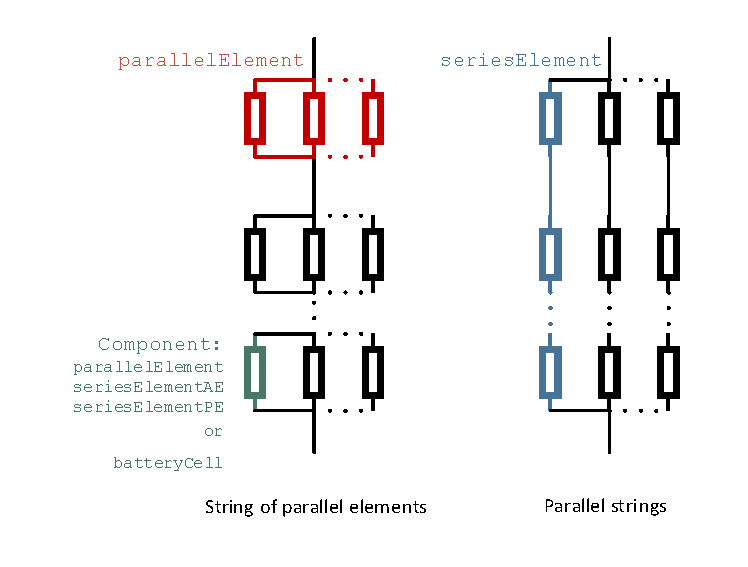
\includegraphics[width=\textwidth]{topologies2.pdf}
	\caption[Visualization of the possible battery topology compositions]{Visualization of the possible battery topology compositions.}
	\label{fig:topologies2}
\end{figure}
Figure~\ref{fig:topologies2} provides a visual overview of the topologies that are possible using different compositions. Using this variation of the Composite design pattern, the components can be combined in any possible way at runtime. The most common battery topologies are strings of parallel elements (SP) and parallel strings of cells (PS)~\cite{cordoba-arenas_control-oriented_2015}. In Figure~\ref{fig:topologies2}, these would be the case if the composition's leaf nodes (cells) were all in the second layer (marked green). However, since every component can be either a cell or another composite, more complicated topologies are made possible in this package. \\
\begin{figure}[t!]
	\captionsetup{type=figure}
	\centering
	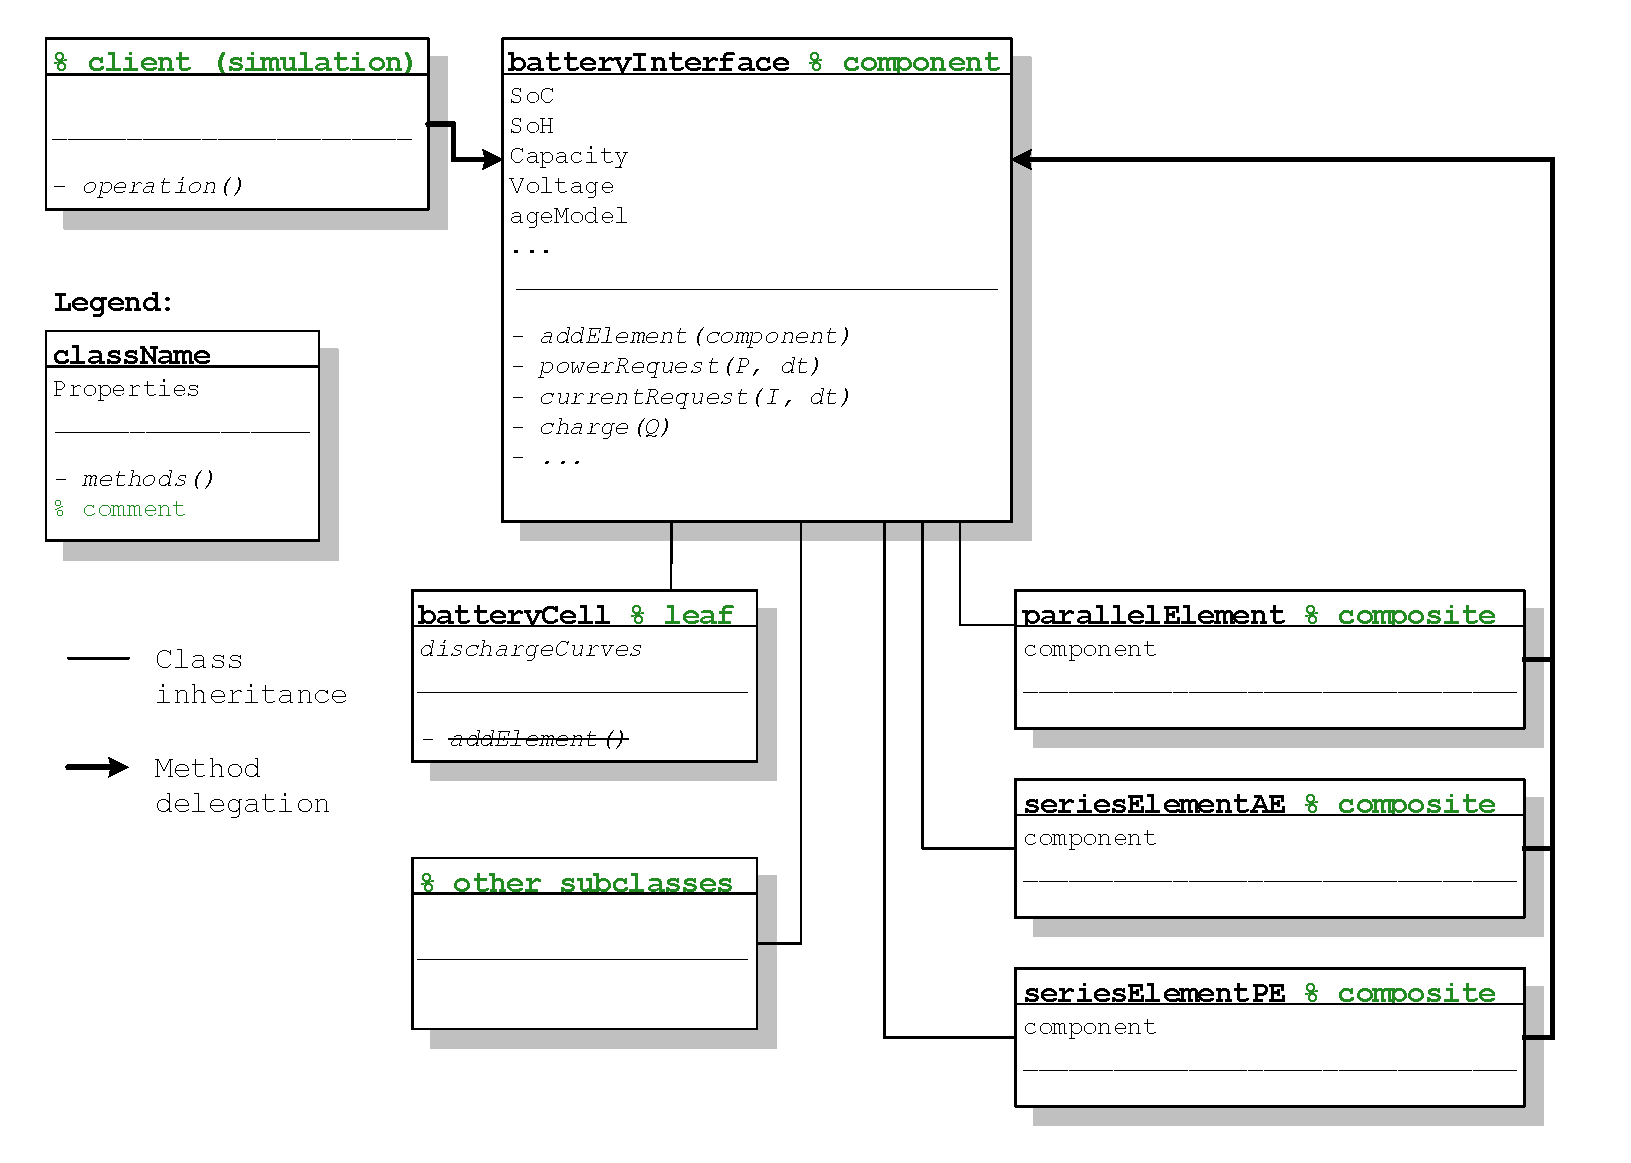
\includegraphics[width=\textwidth]{composite_schema.pdf}
	\caption[Class diagram of the battery composition with communication flows and inheritance links]{Class diagram of the battery composition with communication flows and inheritance links.}
	\label{fig:composite_schema}
\end{figure}

\subsection{Method delegation}
A pattern diagram of the classes used for the topology composition is depicted in Figure~\ref{fig:composite_schema}. Every composite element holds a reference to a component and delegates the methods called on it to said component. The delegated methods are wrapped with the rules of the respective topology in a similar fashion as is done with the Decorator design pattern. An example of the method delegation for a PS configuration - a \mcode{parallelElement} that holds a set of \mcode{seriesElement} objects, each in turn holding a set of \mcode{batteryCell} objects - is visualized in Figure~\ref{fig:method_delegation}. In this example, a current \mcode{I} and the simulation time step size is passed to the \mcode{parallelElement} via a \mcode{getVoltage()} method. The \mcode{parallelElement} determines which portion of \mcode{I} to send to each of it's components and delegates the method. Each \mcode{seriesElement} does the same and delegates the method to it's \mcode{batteryCell} objects. These return their voltages back to the \mcode{seriesElement} objects, which sum up the results received from their cells and pass the sum back to the \mcode{parallelElement}. Finally, the \mcode{parallelElement} calculates the mean of all the summed up voltages it received and passes the end-result back to the client.
\begin{figure}[t!]
	\captionsetup{type=figure}
	\centering
	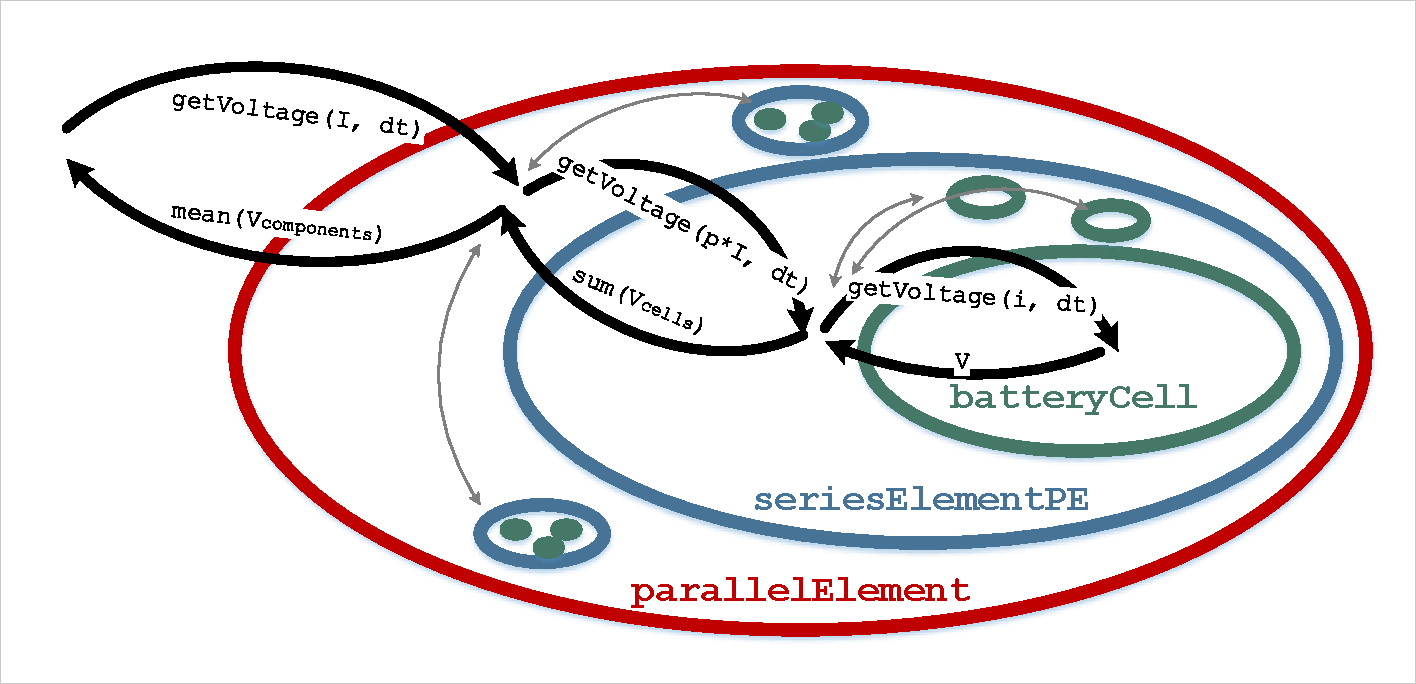
\includegraphics[width=\textwidth]{method_delegation.pdf}
	\caption[Example of a method being delegated across a battery pack composition]{Example of a method being delegated across a battery pack composition.}
	\label{fig:method_delegation}
\end{figure}
The following operations are delegated by an object that implements the \mcode{batteryInterface}:
\begin{itemize}
	\item Determination of the new voltage after charging or discharging a with a certain current and time step size. This is delegated to each \mcode{batteryCell} object's \mcode{dischargeCurves} reference.
	\item Charging or discharging the battery.
	\item Determining the state of the battery if it were to be charged or discharged.
	\item Determining the maximum charging or discharging current.
	\item Calculating the pack's $SoH$.
	\item Getters and setters for the component's voltage and capacity properties.
	\item Getter for the component's internal impedance. 
\end{itemize}
With the number of subcomponents $n$, a component's voltage is determined as
\begin{equation} 
V\subi{component} = \left\lbrace
\begin{smallmatrix}
\frac{\sum_{i=1}^{n}V\subs{subcomponent}{i}}{n} & \text{for a parallel element}\\
& \\
\sum_{i=1}^{n}V\subs{subcomponent}{i} & \text{for a series element} \\
\end{smallmatrix}
\right.
\end{equation}
And a component's capacity is
\begin{equation}
C\subi{component} = \left\lbrace
\begin{smallmatrix}
\sum_{i=1}^{n}C\subs{subcomponent}{i} & \text{for a parallel element}\\
& \\
\min_{i=1}^{n}C\subs{subcomponent}{i} & \text{for a series element with passive equalization} \\
& \\
\frac{\sum_{i=1}^{n}C\subs{subcomponent}{i}}{n} & \text{for a series element with active equalization}\\
\end{smallmatrix}
\right.
\end{equation}
Since the $SoH$ is derived directly from the capacity (see Equation~\ref{eq:age_soh}), a component's $SoH$ can be determined in the same fashion.
\begin{equation}
SoH\subi{component} = \left\lbrace
\begin{smallmatrix}
\sum_{i=1}^{n}SoH\subs{subcomponent}{i} & \text{for a parallel element}\\
& \\
\min_{i=1}^{n}SoH\subs{subcomponent}{i} & \text{for a series element with passive equalization} \\
& \\
\frac{\sum_{i=1}^{n}SoH\subs{subcomponent}{i}}{n} & \text{for a series element with active equalization}\\
\end{smallmatrix}
\right.
\end{equation}
Due to the fact that the model is based on curve fits, the internal impedance $Z\subi{i}$ property is not used for modelling the charging behaviour directly. It does however, determine how the voltages and currents are distributed across the subcomponents when charging or discharging. The impedance proportionality factor $p\subi{z}$ of a subcomponent with index $j$ is the component's $Z\subi{i}$ divided by the sum of all subcomponents' $Z\subi{i}$.
\begin{equation}
p\subs{z}{j} = \frac{Z\subs{i}{j}}{\sum_{i=1}^{n}Z\subs{i}{i}}
\end{equation}
When charging, a series element with active equalization will distribute it's voltage equally across all of it's subcomponents to account for balancing, while a series element with passive equalization will distribute it's voltage according to $p\subs{z}{j}$. For a parallel element, the current is distributed in such a way that the subcomponent $j$ with the lowest $Z\subi{i}$ receives the highest current.
\begin{equation}
I\subs{subcomponent}{j} = \frac{\frac{1}{p\subs{z}{j}}}{\sum_{i=1}^{n}\frac{1}{p\subs{z}{i}}}
\cdot I\subi{component}
\end{equation}


\subsection{Battery Interface}
The battery interface is described in the following subsections. Every component implements the \mcode{batteryInterface}, so the methods described in this section can be called on \mcode{batteryCell} objects and on the composites.

\subsubsection{Battery object initialization}
To initialize a battery object at runtime, the nominal capacity $C\subi{n}$ in Ah and the nominal voltage $V\subi{n}$ in V must be passed to a \mcode{batteryCell} constructor. A composite can be initialized as an "empty" circuit element and the cell (or other composites) can be added to it via it's \mcode{addElements()} method\footnote{Here, "empty" is referred to in the sense of not holding any cells, not in the sense of an empty \matlab\ variable.}.

\begin{lstlisting}
% Initialize an "empty" parallel element
bat = parallelElement;
Cn = 3; % Nominal cell capacity in Ah
Vn = 3.2; % Nominal cell voltage in V
% Initialize 3 battery cells and add them to bat
for i = 1:3
	b = batteryCell(Cn, Vn);
	bat.addElements(b);
end
\end{lstlisting}
The \mcode{addElements()} method also accepts component arrays...
\begin{lstlisting}
for i = 1:3
	b(i) = batteryCell(Cn, Vn);
end
bat.addElements(b);
\end{lstlisting}
...and multiple inputs:
\begin{lstlisting}
b1 = batteryCell(Cn, Vn);
b2 = batteryCell(Cn, Vn);
b3 = batteryCell(Cn, Vn);
bat.addElements(b1, b2, b3);
\end{lstlisting}
To create a composition like the example in Figure~\ref{fig:method_delegation} (see also Figure~\ref{fig:topologies2}, right), the following syntax could be used:
\begin{lstlisting}
% Initialize "empty" parallel element
bat = parallelElement;
% Initialize 3 "empty" series elements each holding 3 cells
for i = 1:3
	se = seriesElementPE; % passive equalization
	for j = 1:3
		se.addElements(batteryCell(Cn, Vn))
	end
	% Add series elements to bat
	bat.addElements(se)
end
% Further initialization operations, e.g. bat.addcurves() here...
\end{lstlisting}

\subsubsection{Battery charging and discharging}
Battery charging \footnote{Discharging will also be referred to as charging (with a negative current) in this documentation.} is handled by the methods \mcode{powerRequest()} and \mcode{currentRequest()}. Both functions are called in a similar manner. The syntax is as follows:
\begin{lstlisting}
[P, V, I] = bat.powerRequest(P, dt);
[P, V, I] = powerRequest(bat, P, dt); % equivalent
[P, V, I] = bat.currentRequest(I, dt);
[P, V, I] = currentRequest(b, I, dt); % equivalent
\end{lstlisting}
Where \mcode{P} is the requested power $P$ in W, \mcode{I} is the requested current $I$ in A and \mcode{dt} is the simulation time step size $\Delta t\subi{s}$ in s. The methods return the actual power throughput in W, the battery's voltage $V$ at the end of the time step and the actual current throughput in A. The returned power and current is limited by the $SoC$ or the cells' maximum currents, among other factors.
\begin{figure}[b!]
	\captionsetup{type=figure}
	\centering
	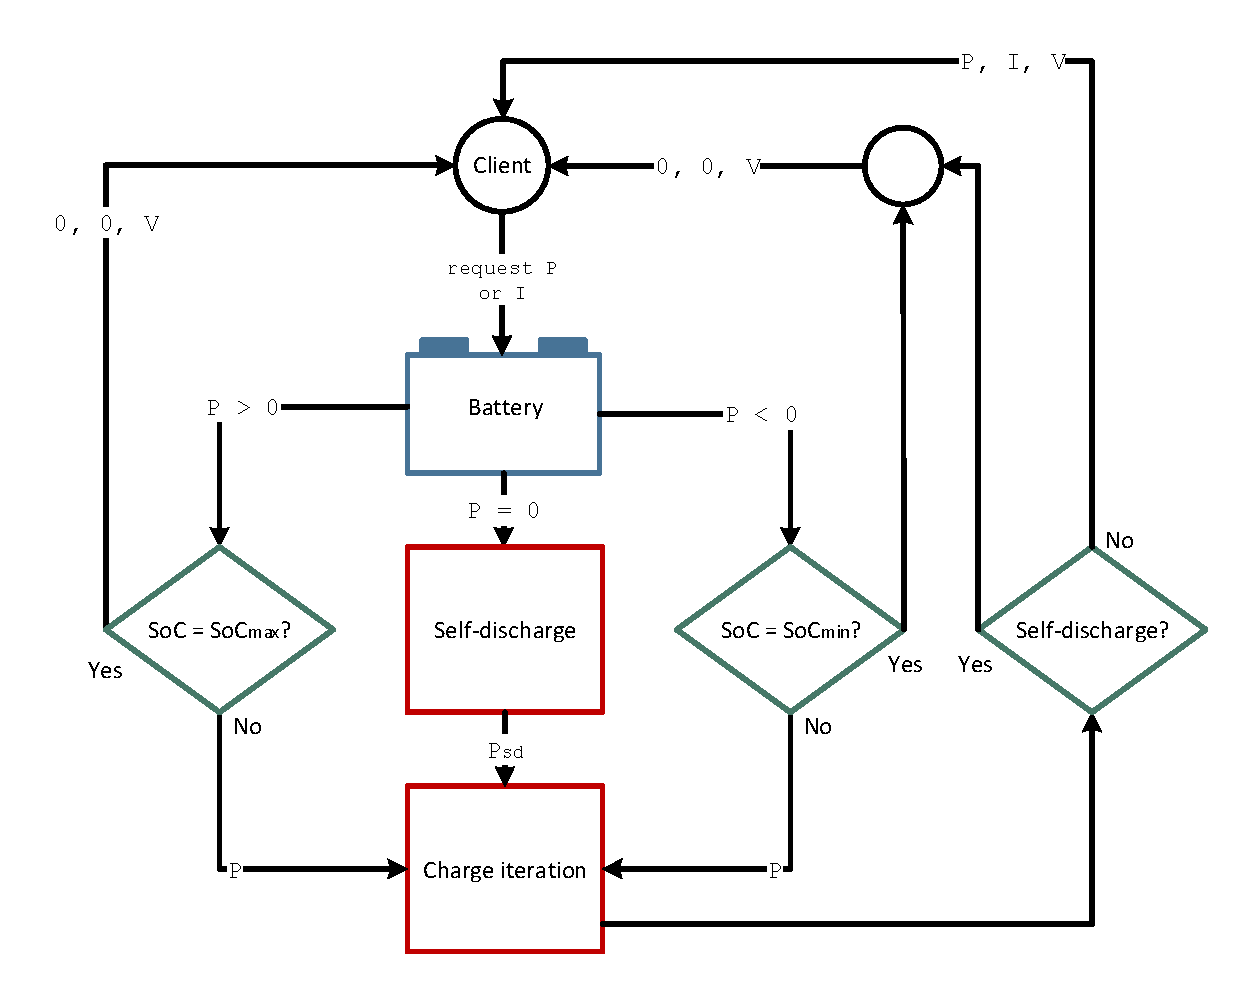
\includegraphics[width=\textwidth]{powerRequest.pdf}
	\caption[Flow chart of the \mcode{powerRequest()} and \mcode{currentRequest()} methods]{Flow chart of the \mcode{powerRequest()} and \mcode{currentRequest()} methods.}
	\label{fig:powerRequest}
\end{figure}
Figure~\ref{fig:powerRequest} contains a flow chart of the charging process. The client sends a request to the battery. If the requested power is not equal to zero and the battery's $SoC$ is not already at it's upper or lower limit, a charge iteration is performed (the \mcode{iteratePower()} and \mcode{iterateCurrent()} methods are called, respectively) and the resulting power, current and voltage are returned to the client. A positive input to the charge iteration  indicates charging and a negative input specifies discharging. If the request is zero, signalling that the battery is in an idle state, a logical flag is set to true and the charge iteration is called with the battery's self-discharge $P\subi{sd}$. The logical flag is checked after every call to the charge iteration methods in order to return a power and current of zero to the client if it was set to true. If the $SoC$ is either at it's upper or lower limit, the battery simply returns it's voltage along with a power and current of zero.\\
\begin{figure}[t!]
	\captionsetup{type=figure}
	\centering
	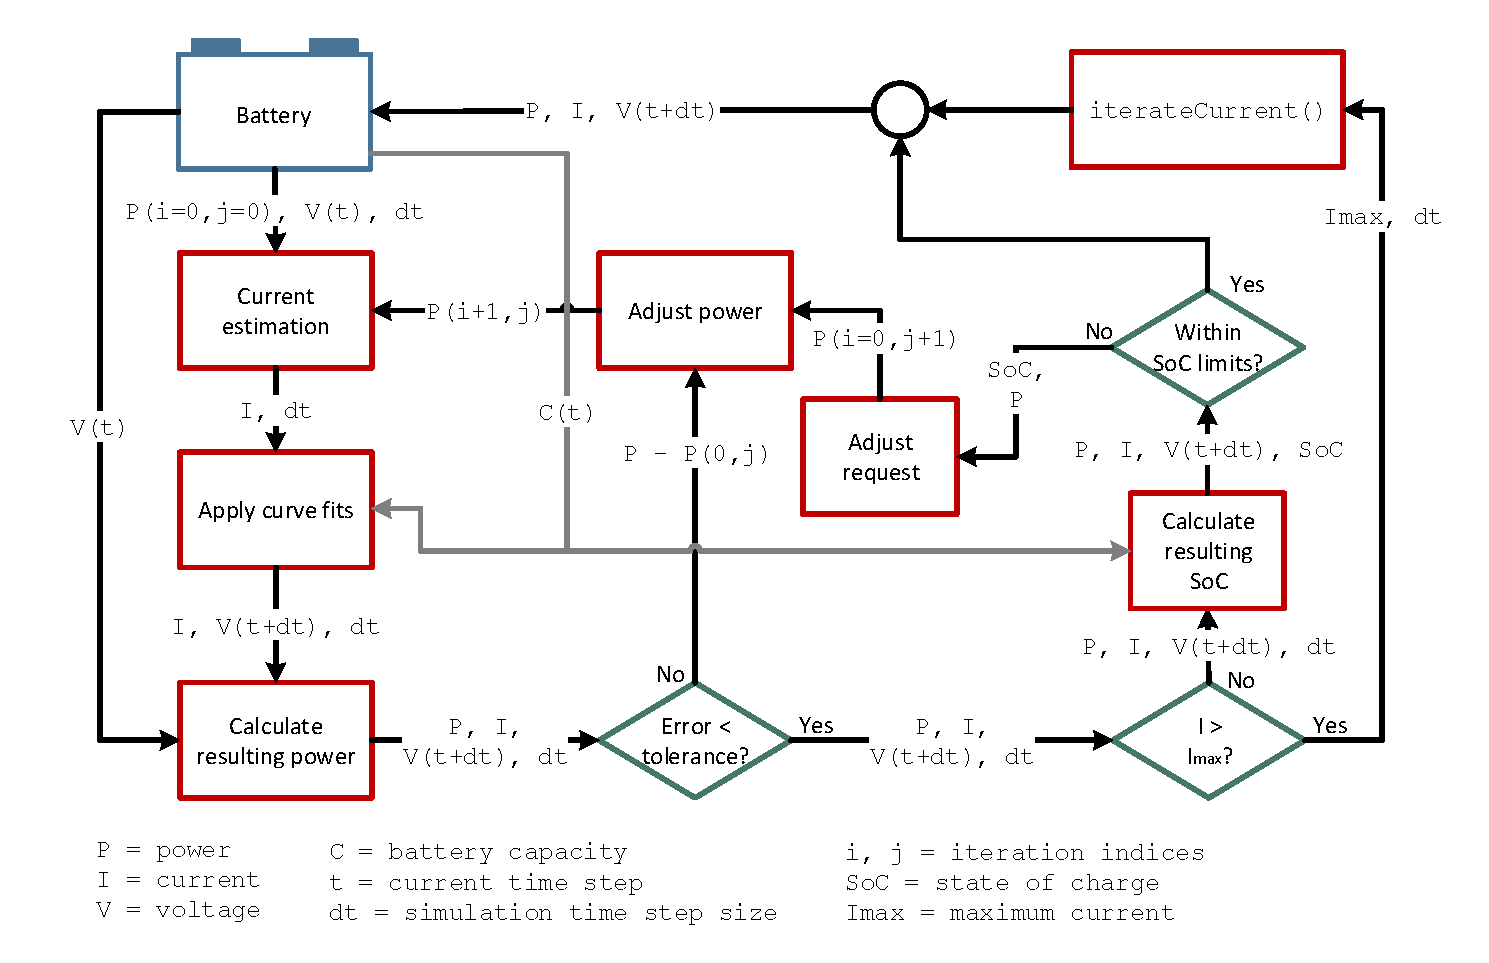
\includegraphics[width=\textwidth]{iteratePower.pdf}
	\caption[Flow chart of the \mcode{iteratePower()} method]{Flow chart of the \mcode{iteratePower()} method.}
	\label{fig:iteratePower}
\end{figure}
A flow chart of the \mcode{iteratePower()} method is depicted in Figure~\ref{fig:iteratePower}. First, a current is estimated from the requested power and the battery's voltage. The current and the time step size are then delegated to the battery cells' \mcode{dischargeCurves} objects, in order to determine the resulting voltage. An approximation of the power is determined from the mean of the returned voltage and the battery's old voltage. This is repeated through recursion until the difference between the iterated power and the originally requested power meets a certain tolerance. If the resulting current is greater than the battery's maximum current $I\subi{max}$, the \mcode{iterateCurrent()} method is called using $I\subi{max}$ as an input. It's output current, the resulting power and voltage are returned. Otherwise, the $SoC$ is determined and compared the battery's upper and lower limit. If the $SoC$ is within the interval $[SoC\subi{min}, SoC\subi{max}]$, the power, current and voltage are returned. Otherwise, the requested power is adjusted according to the difference between the $SoC$ and the respective limit that was exceeded, thus starting the iteration again. \\
\begin{figure}[t!]
	\captionsetup{type=figure}
	\centering
	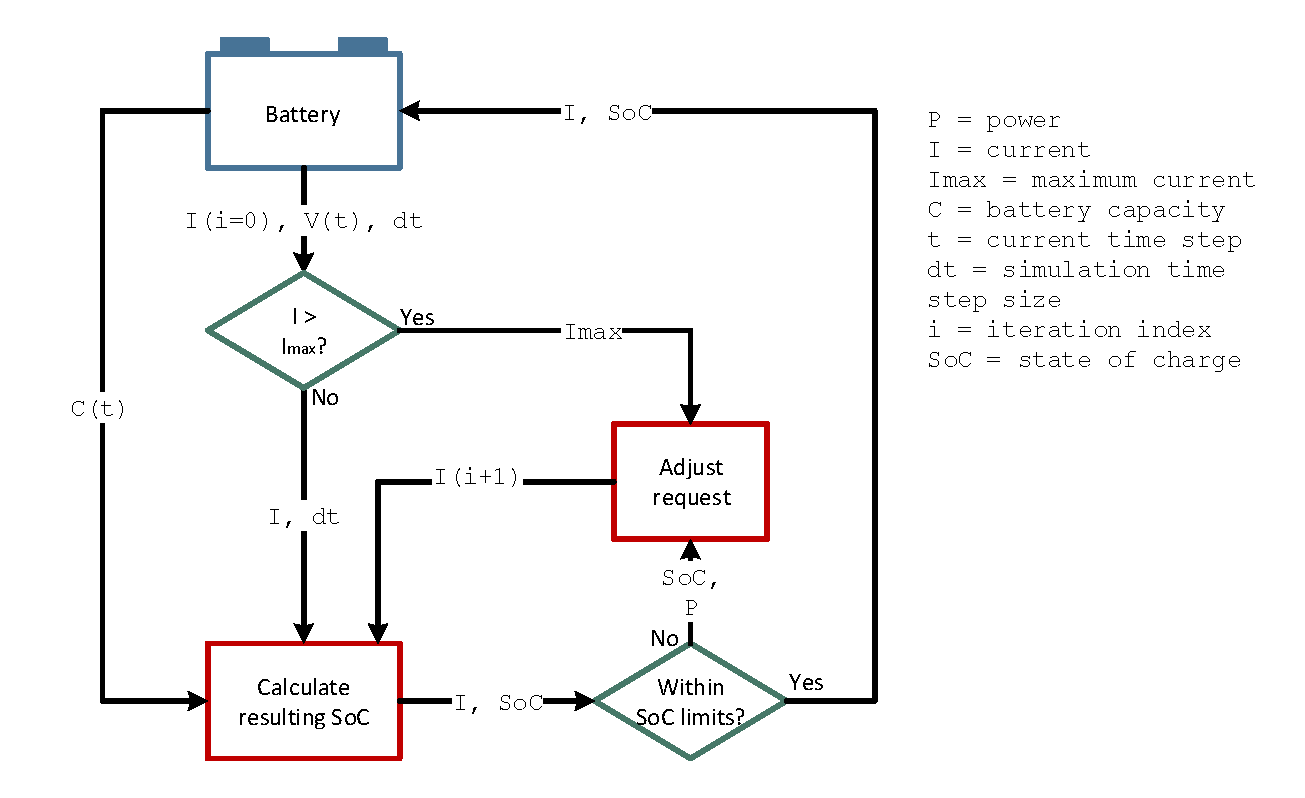
\includegraphics[width=\textwidth]{iterateCurrent.pdf}
	\caption[Flow chart of the \mcode{iterateCurrent()} method]{Flow chart of the \mcode{iterateCurrent()} method.}
	\label{fig:iterateCurrent}
\end{figure}
Figure~\ref{fig:iterateCurrent} depicts a flow chart of the \mcode{iterateCurrent()} function. Using this method is a lot faster than using the \mcode{iteratePower()} function, due to it's comparative simplicity. However, the current may need to be determined separately in some cases. Before the iteration, the current is limited to $I\subi{max}$. Finally, the another limitation is performed if the $SoC$ is not within the interval $[SoC\subi{min}, SoC\subi{max}]$. Normally, one or two iterations should suffice for returning the current and $SoC$. The voltage and power are not calculated and must be determined by calling the \mcode{getNewVoltage()} method if required\footnote{For example, this is done within the \mcode{currentRequest()} method, which does return the voltage and power.}.
%TODO: iteratePower() description
%TODO: iterateCurrent() description
%TODO: Figure showing "jumps" in the voltage with variable charging currents
\subsubsection{Age model level}
\markboth{GUI tools}{GUI tools}
\section{GUI tools}
For a quick and easy set-up of a battery model, two GUI tools were created as part of this package. Since both tools are based on \java\ Swing, a \java\ virtual machine (JVM) must be installed for the GUI tools to function. Normally, \matlab\ comes pre-bundled with a JVM. However, in the rare cases in which this is not the case, an error message is printed to the command window.

\subsection{Battery Pack Designer}
The Battery Pack Designer is a GUI that enables the creation of a \mcode{batteryPack} object. It can be started by typing
\begin{lstlisting}
batteryPack.GUI
\end{lstlisting}
into the command window. Figure~\ref{fig:Designer} shows a screenshot of the tool in Windows. Usage of the tool should be self-explanatory. Detailed information is provided using tool tips, which appear when hovering over GUI element (i.e. button or text field) with the mouse. When the model is fully configured, a \mcode{batteryPack} object can be created and sent to the workspace. The Battery Pack Designer provides a comfortable way to create models for users who are new to the package. It can be practicable for the purpose of getting to know the model and it's interface. \\
However, it is not recommended to save the created objects in MAT files for later use in simulations. Object links within the model (i.e. the link between the age model and the pack; see section~\ref{sec:ageModel}) are broken upon saving, which may result in unexpected behaviour of the loaded objects. 
\begin{figure}[b!]
	\captionsetup{type=figure}
	\centering
	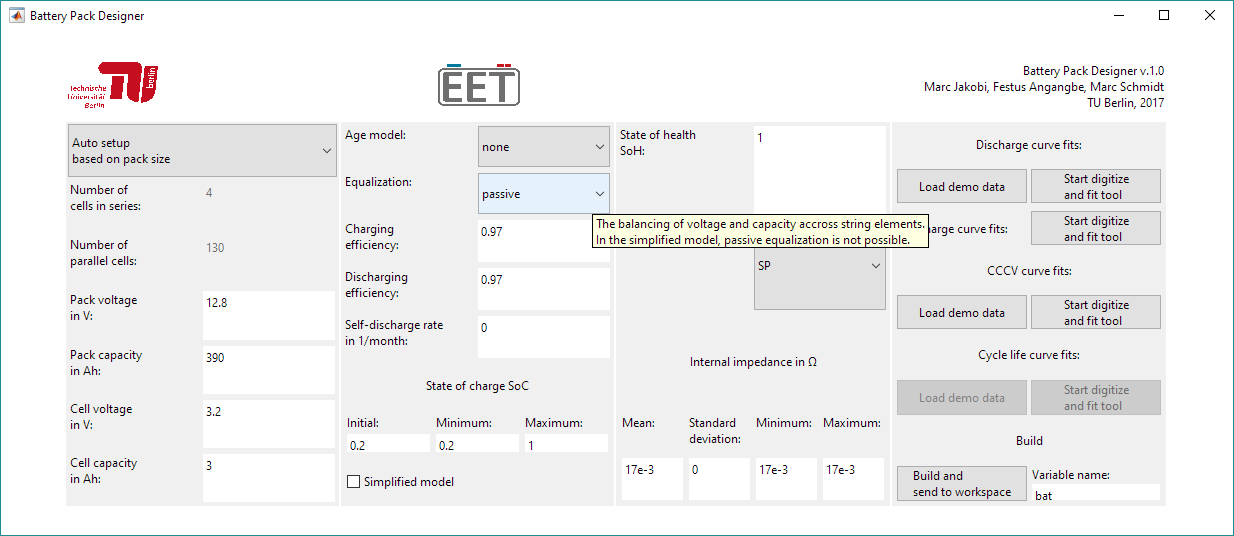
\includegraphics[width=\textwidth]{Designer.png}
	\caption[Screenshot of the Battery Pack Designer in Windows]{Screenshot of the Battery Pack Designer in Windows.}
	\label{fig:Designer}
\end{figure}
Furthermore, if multiple battery cells hold references to a single \mcode{dischargeCurves} object (see section~\ref{sec:dischargeCurvesMain}), the object is deep-copied across all of the cells, potentially resulting in large amounts of data\footnote{This can be fixed by re-adding the \mcode{dischargeCurves} using the \mcode{addcurves()} method after loading.}. The creation of deep-copies upon saving could also lead to memory leaks. Due to this behaviour, it is recommended to initialize the \mcode{batteryPack} at runtime, before the simulation (see section~\ref{sec:batteryPackConstructor}).\\
The Battery Pack Designer contains demo curve fits that can be loaded into the model. Alternatively, user-defined curves can be digitized and fitted using the provided digitizer and curve fit tool, which can be loaded from the Battery Pack Designer or from the command window.

\subsection{Digitizer and curve fit tool}

\markboth{Summary and outlook}{Summary and outlook}
\section{Summary and outlook}
The goal of this project was the development of a flexible, open-source battery pack model that compensates for the dearth of cell-resolved models in the field of battery simulation and can be easily parametrized using data sheets. This was accomplished by means of combining Matlab's highly optimized vectorization and dgemm libraries with OOP design patterns.
A semi-empirical model was successfully developed based on the data sheets of lithium iron phosphate (LFP) cells. Fist, the charging behaviour was replicated using curve fits of measured discharge curves - the cell voltage as functions of the discharged capacity for various currents. These curve fits were combined and used to interpolate the data for currents in between the recorded curves, making it possible to retrieve the voltage for any given current and discharge capacity. The simulated behaviour was validated by removing a measured curve from the data set and comparing it to one that was interpolated using the remaining curve fits. The validated charging behaviour was implemented via the Strategy design pattern, making it possible to swap out the LFP curve fitting classes with user-defined curve fits of other technologies' charging behaviour. A simple event oriented age model was implemented using the Observer design pattern, enabling a loose coupling of the battery pack and age model. This in turn facilitates the implementation of the age model on a cell level and on a simplified pack level as well as the extension with more detailed models that take additional ageing factors into account. A mathematical cycle counting algorithm was implemented and validated by means of comparison with the popular rainflow counting algorithm. \\
The combination of cells into any conceivable topology with either active or passive balancing of strings was made possible with a variation of the Composite design pattern. In order to ensure high performance, method delegation was limited to the components' getters and setters. It was further optimized with caching. By doing so, the actual charge iteration could be implemented on the pack level, rather than having to be realized for each individual cell. A short simulation of a battery pack revealed that it is necessary to differentiate between charging and discharging curves for more realistic behaviour. The ability to do so was implemented in the package. Furthermore, it was shown that a simulation with strongly fluctuating currents results in an equally vigorously oscillating pack voltages. An extension that makes it possible to even out such fluctuations was added to the package.\\ 
Once again using the Observer design pattern, the means for the simulation of CCCV charging combined with a cell-resolved BMS was provided. By limiting the cell-level computation to the setting of a logical flag on the pack level and delegating the charge current calculation to the pack, the workload was minimized. In order to enable more lightweight simulations using this package, a simplified version of the model was devised. Finally, GUI tools and a facade (the \mcode{batteryPack} class) were devised in order to provide the user with a simple interface to the complex subsystems of the model.\\
All in all, the goals set for this project were exceeded. Not only was a model created that can be easily adapted for various technologies. Components of the package can also be used separately and implemented into other models. For a proper validation, it would be necessary to take measurements from a battery in field tests and compare it to a model. This was not possible within the scope of this project due to access and time limitations. However, the test simulations provide a sufficient validation for many use cases. With the fast development of new lithium ion technologies, flexible, easily adaptable models are becoming more and more important. The package developed in the scope of this project provides a good solution. By making the source code freely accessible on GitHub\footnote{Available at: \url{https://github.com/MrcJkb/lfpBattery.git}}, further optimization and validation is facilitated.
\clearpage

\markboth{BSD license}{BSD license}
\section*{BSD license}
\addcontentsline{toc}{section}{BSD license}
Copyright \textcopyright\ 2017 Marc Jakobi, Festus Anyangbe, Marc Schmidt\newline
All rights reserved.
\newline
\newline
Redistribution and use in source and binary forms, with or without modification, are permitted provided that the following conditions are met:
\newline\newline
1. Redistributions of source code must retain the above copyright notice, this list of conditions and the following disclaimer.
\newline\newline
2. Redistributions in binary form must reproduce the above copyright notice, this list of conditions and the following disclaimer in the documentation and/or other materials provided with the distribution.
\newline\newline
3. Neither the name of the copyright holder nor the names of its contributors may be used to endorse or promote products derived from this software without specific prior written permission.
\newline\newline
THIS SOFTWARE IS PROVIDED BY THE COPYRIGHT HOLDERS AND CONTRIBUTORS "AS IS" AND ANY EXPRESS OR IMPLIED WARRANTIES, INCLUDING, BUT NOT LIMITED TO, THE IMPLIED WARRANTIES OF MERCHANTABILITY AND FITNESS FOR A PARTICULAR PURPOSE ARE DISCLAIMED. IN NO EVENT SHALL THE COPYRIGHT HOLDER OR CONTRIBUTORS BE LIABLE FOR ANY DIRECT, INDIRECT, INCIDENTAL, SPECIAL, EXEMPLARY, OR CONSEQUENTIAL
DAMAGES (INCLUDING, BUT NOT LIMITED TO, PROCUREMENT OF SUBSTITUTE GOODS OR SERVICES; LOSS OF USE, DATA, OR PROFITS; OR BUSINESS INTERRUPTION) HOWEVER CAUSED AND ON ANY THEORY OF LIABILITY, WHETHER IN CONTRACT, STRICT LIABILITY, OR TORT (INCLUDING NEGLIGENCE OR OTHERWISE) ARISING IN ANY WAY OUT OF THE USE OF THIS SOFTWARE, EVEN IF ADVISED OF THE POSSIBILITY OF SUCH DAMAGE.
\addcontentsline{toc}{section}{References}
\printbibliography
%TODO Write summary + conclusion
%TODO correct Fred's thesis from PhD to Masters's in references
%TODO replace umlauts in .bib file
\end{document}